\documentclass[12pt,a4paper,twoside,openright]{report}
\let\openright=\cleardoublepage



%%% Choose a language %%%

\newif\ifEN
\ENtrue   % uncomment this for english
%\ENfalse   % uncomment this for czech

%%% Configuration of the title page %%%

\def\ThesisTitleStyle{mff} % MFF style
%\def\ThesisTitleStyle{cuni} % uncomment for old-style with cuni.cz logo
%\def\ThesisTitleStyle{natur} % uncomment for nature faculty logo

\def\UKFaculty{Faculty of Mathematics and Physics}
%\def\UKFaculty{Faculty of Science}

\def\UKName{Charles University in Prague} % this is not used in the "mff" style

% Thesis type names, as used in several places in the title
% \def\ThesisTypeTitle{\ifEN BACHELOR THESIS \else BAKALÁŘSKÁ PRÁCE \fi}
\def\ThesisTypeTitle{\ifEN MASTER THESIS \else DIPLOMOVÁ PRÁCE \fi}
%\def\ThesisTypeTitle{\ifEN RIGOROUS THESIS \else RIGORÓZNÍ PRÁCE \fi}
%\def\ThesisTypeTitle{\ifEN DOCTORAL THESIS \else DISERTAČNÍ PRÁCE \fi}
% \def\ThesisGenitive{\ifEN bachelor \else bakalářské \fi}
\def\ThesisGenitive{\ifEN master \else diplomové \fi}
% \def\ThesisGenitive{\ifEN rigorous \else rigorózní \fi}
%\def\ThesisGenitive{\ifEN doctoral \else disertační \fi}
% \def\ThesisAccusative{\ifEN bachelor \else bakalářskou \fi}
\def\ThesisAccusative{\ifEN master \else diplomovou \fi}
%\def\ThesisAccusative{\ifEN rigorous \else rigorózní \fi}
%\def\ThesisAccusative{\ifEN doctoral \else disertační \fi}



%%% Fill in your details %%%

% (Note: \xxx is a "ToDo label" which makes the unfilled visible. Remove it.)
\def\ThesisTitle{Graph neural networks and deep reinforcement learning in job scheduling}
\def\ThesisAuthor{Maroš Bratko}
\def\YearSubmitted{2024}

% department assigned to the thesis
\def\Department{Department of Theoretical Computer Science and Mathematical Logic}
% Is it a department (katedra), or an institute (ústav)?
\def\DeptType{Department}

\def\Supervisor{prof. RNDr. Ing. Martin Holeňa, CSc.}
\def\SupervisorsDepartment{Department of Theoretical Computer Science and Mathematical Logic}

% Study programme and specialization
\def\StudyProgramme{Computer Science - Artificial Intelligence (N0619A140003)}
\def\StudyBranch{IUIP (0619TA140003)}

\def\Dedication{%
I want to thank my supervisor, prof. RNDr. Ing. Martin Holeňa, CSc., for his guidance and support throughout writing this thesis. I am also very grateful for our discussions about the academic world, which gave me invaluable insight into my future career decisions.

I want to thank my family, who encouraged and supported me during my studies.

I want to thank my friends, who made my studies enjoyable and happy experience. I want to specifically thank my friend, Daniel B., for being there since the start of college and with whom life is fun.
}

\def\AbstractEN{%
The priority dispatching rule (PDR) is a greedy heuristic algorithm used to obtain approximate solutions to the NP-hard job scheduling problem (JSP). The manual design of PDRs requires domain knowledge to achieve good results. Recently, deep reinforcement learning has been used to automate the process of designing PDRs, where PDRs are formulated as a Markov Decision Process exploiting graph representation of JSP, and a graph neural network (GNN) selects the operations to be dispatched. In this thesis, we present the overview of five models published in literature with their source code publicly available on GitHub and experimentally compare their performance on three different variants of JSP. Our experiments show that the choice of input features, e.g., the amount of remaining work, significantly affects the model's performance regardless of the GNN architecture. This suggests that the feature selection is essential for learning high-quality PDRs.
}

\def\AbstractCS{%
Prioritní rozhodovací pravidla (PDRs) jsou hladové heuristické algoritmy používané ke získaní přibližného řešení NP-těžkého úkolu organizace práce (JSP). Manuální příprava PDR vyžaduje zkušenosti v dané oblasti pro získaní dobrých výsledků. V posledních letech bylo k automatizaci přípravy PDR využito zpětnovazební učení, kde jsou PDR formulováný jako Markovův rozhodovací proces využívajíci grafovou reprezentaci JSP, ve které grafová neurónová síť (GNN) vybírá operace ke spuštění. V této prácí uvádíme přehled pěti modelů publikovaných v literatuře, kterých zdrojové kódy jsou volně dostupné na GitHubu, a experimentálňe porovnáme jejich výsledky. Naše experimentuji ukazují, že volba vstupních příznaků, napr. množství zbývající práce, významně ovlivňuje kvalitu výsledných řešení bez ohledu na architekturu GNN. To naznačuje, že výběr vstupních příznaků je pro přípravu kvalitních PDR zásadní.
}

% 3 to 5 keywords (recommended), each enclosed in curly braces.
% Keywords are useful for indexing and searching for the theses by topic.
\def\Keywords{%
{job-shop scheduling}, {graph neural networks}, {deep reinforcement learning}, {markov decision process}
}

% If your abstracts are long and do not fit in the infopage, you can make the
% fonts a bit smaller by this setting. (Also, you should try to compress your abstract more.)
% Alternatively, consider increasing the size of the page by uncommenting the
% geometry modification in thesis.tex.
\def\InfoPageFont{}
%\def\InfoPageFont{\small}  %uncomment to decrease font size

\ifEN\relax\else
% If you are writing a czech thesis, you additionally need to fill in the
% english translation of the metadata here!
\def\ThesisTitleEN{\xxx{Thesis title in English}}
\def\DepartmentEN{\xxx{Name of the department in English}}
\def\DeptTypeEN{\xxx{Department}}
\def\SupervisorsDepartmentEN{\xxx{Superdepartment}}
\def\StudyProgrammeEN{\xxx{study programme}}
\def\StudyBranchEN{\xxx{study branch}}
\def\KeywordsEN{%
\xxx{{key} {words}}
}
\fi


\usepackage[a-2u]{pdfx}

\ifEN\else\usepackage[czech,shorthands=off]{babel}\fi

% See https://en.wikipedia.org/wiki/Canons_of_page_construction before
% modifying the size of printable area. LaTeX defaults are great.
% If you feel it would help anything, you can enlarge the printable area a bit:
%\usepackage[textwidth=390pt,textheight=630pt]{geometry}
% The official recommendation expands the area quite a bit (looks pretty harsh):
%\usepackage[textwidth=145mm,textheight=247mm]{geometry}

%%% TYPICAL FONT CHOICES (uncomment what you like) %%%
% Recommended combo: Libertinus (autoselects Biolinum for sans) and everything
% else (math+tt) comes from Latin Modern)
\usepackage{lmodern}
\usepackage[mono=false]{libertinus}

% For the "classic" LaTeX fonts (very good for pure math theses), simply
% comment out the libertinus package above.

% IBM Plex font suite: nice, but requires us to fine-tune the sizes and does
% not directly support small caps (\textsc):
%\usepackage[usefilenames,RM={Scale=0.88},SS={Scale=0.88},SScon={Scale=0.88},TT={Scale=0.88},DefaultFeatures={Ligatures=Common}]{plex-otf}

% TeX Gyre combo (Pagella+Heros+Cursor)
%\usepackage{fontspec}
%\setmainfont{TeX Gyre Pagella}
%\setsansfont{TeX Gyre Heros}
%\setmonofont{TeX Gyre Cursor}

% some useful packages
\usepackage{microtype}
\usepackage{amsmath,amsfonts,amsthm,bm}
\usepackage{graphicx}
\usepackage{xcolor}
\usepackage{booktabs}
\usepackage{caption}
\usepackage{floatrow}

% Bibliography formatting.
% CHECK THE REQUIREMENTS OF YOUR DEPARTMENT AND FACULTY ON THE CITATION FORMAT!
%
% These are relatively "safe" default options that most people use:
\usepackage[natbib,style=numeric,sorting=none]{biblatex}
% alternative with alphanumeric citations (more informative than numbers, and
% more common in computer science journals):
%\usepackage[natbib,style=alphabetic]{biblatex}
%
% ALTERNATIVES THAT CONFORM TO ISO690
% ISO690 is not the greatest citation format ever, but may be formally
% required at Charles University, depending on your faculty and department.
%\usepackage[natbib,style=iso-numeric,sorting=none]{biblatex}
%\usepackage[natbib,style=iso-alphabetic]{biblatex}
% You might want to add extra options such as `maxbibnames=6,maxcitenames=2`
% here to further conform to some of the formatting requirements (see below for
% details). Again, consult your faculty rules.
%
% Additional option choices:
%  - add `giveninits=true` to typeset "E. A. Poe" instead of full Edgar Allan
%  - `terseinits=true` additionaly shortens it to nature-like "Poe EA"
%  - add `maxnames=10` to limit (or loosen) the maximum number of authors in
%    bibliography entry before shortening to `et al.` (useful when referring to
%    book collections that may have hundreds of authors)
%  - use `maxcitenames=2` to finetune the amount of authors listed in text-cite
%    commands (\citet). Corresponding option that only affects the bibliography
%    is `maxbibnames=10`.
%  - `sorting=none` causes the bibliography list to be ordered by the order of
%    citation as they appear in the text, which is usually the desired behavior
%    with numeric citations. Additionally you can use a style like
%    `numeric-comp` that compresses the long lists of citations such as
%    [1,2,3,4,5,6,7,8] to simpler [1--8]. This is especially useful if you plan
%    to add tremendous amounts of citations, as usual in life sciences and
%    bioinformatics.
%  - if you don't like the "In:" appearing in the bibliography, use the
%    extended style (`ext-numeric` or `ext-alphabetic`), and add option
%    `articlein=false`.
%
% possibly reverse the names of the authors with the default styles:
%\DeclareNameAlias{default}{family-given}

% load the file with bibliography entries
\addbibresource{refs.bib}

% remove this if you won't use fancy verbatim environments
\usepackage{fancyvrb}

% remove this if you won't typeset TikZ graphics
\usepackage{tikz}
\usetikzlibrary{positioning} %add libraries as needed (shapes, decorations, ...)

% remove this if you won't typeset any pseudocode
\usepackage{algpseudocode}
\usepackage{algorithm}

% remove this if you won't list any source code
\usepackage{listings}


\hypersetup{unicode}
\hypersetup{breaklinks=true}

\usepackage[noabbrev]{cleveref}


% various forms of TODOs (you should remove this before submitting)
\usepackage[textsize=tiny, backgroundcolor=yellow!25, linecolor=black!25]{todonotes}
\newcommand{\xxx}[1]{\textcolor{red!}{#1}}

 % remove this before compiling the final version


% use this for typesetting a chapter without a number, e.g. intro and outro
\def\chapwithtoc#1{\chapter*{#1}\addcontentsline{toc}{chapter}{#1}}

% If there is a line/figure overflowing into page margin, this will make the
% problem evident by drawing a thick black line at the overflowing spot. You
% should not disable this.
\overfullrule=3mm

% The maximum stretching of a space. Increasing this makes the text a bit more
% sloppy, but may prevent the overflows by moving words to next line.
\emergencystretch=1em

\ifEN
\theoremstyle{plain}
\newtheorem{thm}{Theorem}
\newtheorem{lemma}[thm]{Lemma}
\newtheorem{claim}[thm]{Claim}
\newtheorem{defn}{Definition}
\theoremstyle{remark}
\newtheorem*{cor}{Corollary}
\else
\theoremstyle{plain}
\newtheorem{thm}{Věta}
\newtheorem{lemma}{Lemma}
\newtheorem{claim}{Tvrzení}
\newtheorem{defn}{Definice}
\theoremstyle{remark}
\newtheorem*{cor}{Důsledek}
\fi

\newenvironment{myproof}{
  \par\medskip\noindent
  \textit{\ifEN Proof \else Důkaz \fi}.
}{
\newline
\rightline{$\qedsymbol$}
}

% real/natural numbers
\newcommand{\R}{\mathbb{R}}
\newcommand{\N}{\mathbb{N}}

% asymptotic complexity
\newcommand{\asy}[1]{\mathcal{O}(#1)}

% listings and default lstlisting config (remove if unused)
\DeclareNewFloatType{listing}{}
\floatsetup[listing]{style=ruled}

\DeclareCaptionStyle{thesis}{style=base,font={small,sf},labelfont=bf,labelsep=quad}
\captionsetup{style=thesis}
\captionsetup[algorithm]{style=thesis,singlelinecheck=off}
\captionsetup[listing]{style=thesis,singlelinecheck=off}

% Customization of algorithmic environment (comment style)
\renewcommand{\algorithmiccomment}[1]{\textcolor{black!25}{\dotfill\sffamily\itshape#1}}

% Uncomment for table captions on top. This is sometimes recommended by the
% style guide, and even required for some publication types.
%\floatsetup[table]{capposition=top}
%
% (Opinionated rant:) Captions on top are not "compatible" with the general
% guideline that the tables should be formatted to be quickly visually
% comprehensible and *beautiful* in general (like figures), and that the table
% "head" row (with column names) should alone communicate most of the content
% and interpretation of the table. If you just need to show a long boring list
% of numbers (because you have to), either put some effort into showing the
% data in an attractive figure-table, or move the data to an attachment and
% refer to it, so that the boredom does not impact the main text flow.
%
% You can make the top-captions look much less ugly by aligning the widths of
% the caption and the table, with setting `framefit=yes`, as shown below.  This
% additionally requires some extra markup in your {table} environments; see the
% comments in the example table in `ch2.tex` for details.
%\floatsetup[table]{capposition=top,framefit=yes}

\ifEN\floatname{listing}{Listing}
\else\floatname{listing}{Výpis kódu}\fi
\lstset{ % use this to define styling for any other language
  language=C++,
  tabsize=2,
  showstringspaces=false,
  basicstyle=\footnotesize\tt\color{black!75},
  identifierstyle=\bfseries\color{black},
  commentstyle=\color{green!50!black},
  stringstyle=\color{red!50!black},
  keywordstyle=\color{blue!75!black}}

% Czech versions of the used cleveref references (It's not as convenient as in
% English because of declension, cleveref is limited to sg/pl nominative. Use
% plain \ref to dodge that.)
\ifEN\relax\else
\crefname{chapter}{kapitola}{kapitoly}
\Crefname{chapter}{Kapitola}{Kapitoly}
\crefname{section}{sekce}{sekce}
\Crefname{section}{Sekce}{Sekce}
\crefname{subsection}{sekce}{sekce}
\Crefname{subsection}{Sekce}{Sekce}
\crefname{subsubsection}{sekce}{sekce}
\Crefname{subsubsection}{Sekce}{Sekce}
\crefname{figure}{obrázek}{obrázky}
\Crefname{figure}{Obrázek}{Obrázky}
\crefname{table}{tabulka}{tabulky}
\Crefname{table}{Tabulka}{Tabulky}
\crefname{listing}{výpis}{výpisy}
\Crefname{listing}{Výpis}{Výpisy}
\floatname{algorithm}{Algoritmus}
\crefname{algorithm}{algoritmus}{algoritmy}
\Crefname{algorithm}{Algoritmus}{Algoritmy}
\newcommand{\crefpairconjunction}{ a~}
\newcommand{\crefrangeconjunction}{ a~}
\fi
 % use this file for various custom definitions


\begin{document}

% the layout is mandatory, edit only in dire circumstances

\pagestyle{empty}
\hypersetup{pageanchor=false}
\begin{center}

% top part of the layout, this actually differs between faculties

\def\ThesisTitleXmff{%
  \ifEN
    \centerline{\mbox{
\includegraphics[width=166mm]{img/logo-en.pdf}}}
  \else
    \centerline{\mbox{
\includegraphics[width=166mm]{img/logo-cs.pdf}}}
  \fi
  \vspace{-8mm}\vfill%
  {\bf\Large\ThesisTypeTitle}
  \vfill%
  {\LARGE\ThesisAuthor}\par
  \vspace{15mm}%
  {\LARGE\bfseries\ThesisTitle}
  \vfill%
  \Department}
\def\ThesisTitleCuniLogo#1{%
  {\large\UKName\par\medskip\par\UKFaculty }
  \vfill%
  {\bf\Large\ThesisTypeTitle}
  \vfill%
  \includegraphics[width=70mm]{#1}
  \vfill%
  {\LARGE\ThesisAuthor}\par
  \vspace{15mm}%
  {\LARGE\bfseries\ThesisTitle}
  \vfill%
  \Department\par}
\def\ThesisTitleXcuni{\ThesisTitleCuniLogo{img/uklogo.pdf}}
\def\ThesisTitleXnatur{\ThesisTitleCuniLogo{img/naturlogo.pdf}}

% choose the correct page and print it
\csname ThesisTitleX\ThesisTitleStyle\endcsname
% latex corner: X is the new @

\vfill

{
\centerline{\vbox{\halign{\hbox to 0.45\hsize{\hfil #}&\hskip 0.5em\parbox[t]{0.45\hsize}{\raggedright #}\cr
\ifEN Supervisor of the \ThesisGenitive thesis:
\else Vedoucí \ThesisGenitive práce: \fi
& \Supervisor \cr
\noalign{\vspace{2mm}}
\ifEN Study programme: \else Studijní program: \fi
& \StudyProgramme \cr
}}}}

\vfill

\ifEN Prague \else Praha \fi
\YearSubmitted

\end{center}

\newpage

% remember to sign this!
\openright
\hypersetup{pageanchor=true}
\pagestyle{plain}
\pagenumbering{roman}
\vglue 0pt plus 1fill

\ifEN
\noindent
I declare that I carried out this master thesis on my own, and only with the
cited sources, literature and other professional sources.
\else
\noindent
Prohlašuji, že jsem tuto \ThesisAccusative práci vypracoval(a) samostatně a výhradně
s~použitím citovaných pramenů, literatury a dalších odborných zdrojů.
Tato práce nebyla využita k získání jiného nebo stejného titulu.
\fi

\ifEN
\medskip\noindent
I understand that my work relates to the rights and obligations under the Act No. 121/2000 Sb., the
Copyright Act, as amended, in particular the fact that the Charles University has
the right to conclude a license agreement on the use of this work as a school work
pursuant to Section 60 subsection 1 of the Copyright Act.
\else
\medskip\noindent
Beru na~vědomí, že se na moji práci vztahují práva a povinnosti vyplývající
ze zákona č. 121/2000 Sb., autorského zákona v~platném znění, zejména skutečnost,
že Univerzita Karlova má právo na~uzavření licenční smlouvy o~užití této
práce jako školního díla podle §60 odst. 1 autorského zákona.
\fi

\vspace{10mm}


\ifEN
\hbox{\hbox to 0.5\hsize{%
In \hbox to 6em{\dotfill} date \hbox to 6em{\dotfill}
\hss}\hbox to 0.5\hsize{\dotfill\quad}}
\smallskip
\hbox{\hbox to 0.5\hsize{}\hbox to 0.5\hsize{\hfil Author's signature\hfil}}
\else
\hbox{\hbox to 0.5\hsize{%
V \hbox to 6em{\dotfill} dne \hbox to 6em{\dotfill}
\hss}\hbox to 0.5\hsize{\dotfill\quad}}
\smallskip
\hbox{\hbox to 0.5\hsize{}\hbox to 0.5\hsize{\hfil Podpis autora\hfil}}
\fi

\vspace{20mm}
\newpage

% dedication

\openright

\noindent
\Dedication

\newpage

% mandatory information page

\openright

\vbox to 0.49\vsize{\InfoPageFont
\setlength\parindent{0mm}
\setlength\parskip{5mm}

\ifEN Title: \else Název práce: \fi
\ThesisTitle

\ifEN Author: \else Autor: \fi
\ThesisAuthor

\DeptType:
\Department

\ifEN Supervisor: \else Vedoucí \ThesisGenitive práce: \fi
\Supervisor, \SupervisorsDepartment

\ifEN Abstract: \AbstractEN \else Abstrakt: \AbstractCS \fi

\ifEN Keywords: \else Klíčová slova: \fi
\Keywords

\vss}\ifEN\relax\else\nobreak\vbox to 0.49\vsize{\InfoPageFont
\setlength\parindent{0mm}
\setlength\parskip{5mm}

Title:
\ThesisTitleEN

Author:
\ThesisAuthor

\DeptTypeEN:
\DepartmentEN

Supervisor:
\Supervisor, \SupervisorsDepartmentEN

Abstract:
\AbstractEN

Keywords:
\KeywordsEN

\vss}
\fi

\newpage

\vbox to 0.49\vsize{\InfoPageFont
\setlength\parindent{0mm}
\setlength\parskip{5mm}


Název práce: Grafové neuronové sítě a hluboké posilované učení při rozvrhování prací

Autor: Maroš Bratko

Katedra: Katedra teoretické informatiky a matematické logiky

Vedoucí diplomové práce: prof. RNDr. Ing. Martin Holeňa, CSc.

Abstrakt: Prioritní rozhodovací pravidla (PDRs) jsou hladové heuristické algoritmy používané ke získaní přibližného řešení NP-těžkého úkolu organizace práce (JSP). Manuální příprava PDR vyžaduje zkušenosti v dané oblasti pro získaní dobrých výsledků. V posledních letech bylo k automatizaci přípravy PDR využito zpětnovazební učení, kde jsou PDR formulováný jako Markovův rozhodovací proces využívajíci grafovou reprezentaci JSP, ve které grafová neurónová síť (GNN) vybírá operace ke spuštění. V této prácí uvádíme přehled pěti modelů publikovaných v literatuře, kterých zdrojové kódy jsou volně dostupné na GitHubu, a experimentálňe porovnáme jejich výsledky. Naše experimentuji ukazují, že volba vstupních příznaků, napr. množství zbývající práce, významně ovlivňuje kvalitu výsledných řešení bez ohledu na architekturu GNN. To naznačuje, že výběr vstupních příznaků je pro přípravu kvalitních PDR zásadní.

Klíčová slova: organizace práce, grafové neurónové sítě, hluboké zpětnovazební učení, Markovův rozhodovací proces

\vss}

\newpage

\openright
\pagestyle{plain}
\pagenumbering{arabic}
\setcounter{page}{1}


\tableofcontents


\chapwithtoc{Introduction}

Job scheduling considers the optimal allocation of a number of jobs consisting of multiple operations with predefined constraints (e.g., operations are processed in a 
specific order) to a set of shared resources to minimize total makespan, tardiness, cost, or other objectives \cite{YamadaNakanoJSSP}. Each resource can process only one operation at a time and is non-preemptive, i.e., it runs without interruption.
\par
Different constraints and conditions lead to different variants of job scheduling. 
Job shop scheduling problem assumes all jobs to be known apriori and that each operation can be allocated only to one given machine \cite{YamadaNakanoJSSP}. In flexible job-shop scheduling, each operation can be allocated to any of the machines from a given subset of machines \cite{DAUZEREPERES2024409}. Dynamic job-shop scheduling (DJSP), one of the more common variants at the time, tackles the stochastic aspects of modern manufacturing, e.g., the arrival of new jobs during the execution of the schedule or uncertain processing time \cite{MOHAN201934}.
\par
Due to the NP-hardness of these problems \cite{Garey1976TheCO}, numerous approaches and heuristics have been proposed over time to yield approximate solutions \cite{Jansen2000ApproximationAF}. Extensively studied meta-heuristics for job scheduling include genetic algorithms \cite{PEZZELLA20083202, zhang2011effective}, tabu search \cite{Brandimarte_1993}, memetic algorithms \cite{frutos2010memetic}, particle swarm optimization \cite{ZHANG20091309}, and simulated annealing \cite{Yamada1996}.
\par
Priority dispatching rule (PDR) \cite{Haupt1989ASO} is a computationally fast and intuitive heuristic method compared to other optimization methods and is widely used in scheduling systems. Many different PDRs have been proposed and extensively studied in the literature \cite{doi:10.1080/00207543.2011.611539}. Designing a quality PDR is usually a very time-consuming task requiring extensive domain knowledge. Deep reinforcement learning has already been proposed as a possible solution for the automatization of algorithm learning for combinatorial optimization problems \cite{bengio2020machine}. Several recent works have focused on extending this technique to job scheduling \cite{zhang2020learning, https://doi.org/10.1002/tee.23788, DBLP:journals/corr/abs-2106-01086, 10114974, 9826438, 10226873} applying graph neural networks on a graph representation of job scheduling problems \cite{BLAZEWICZ2000317}.\\
\par
This presents the overview of five publicly available models for solving job shop scheduling using graph neural networks and deep reinforcement learning. In \textbf{Chapter 1}, we define job shop scheduling problems and their variants. We also describe priority dispatching rules, how they are used in the context of job shop scheduling, and how their design can be automated using reinforcement learning. In \textbf{Chapter 2}, we introduce the concept of graph neural networks and deep reinforcement learning. We discuss different neural architectures and training algorithms. In \textbf{Chapter 3}, we present five publicly available models found in the literature and on GitHub. In \textbf{Chapter 4}, we experimentally compare these models and present the results. In \textbf{Chapter 5}, we interpret the results of our experiments.
\chapter{Job scheduling}
\label{chap:refs}

Job scheduling allocates jobs to machines. There are many different variants of job scheduling, each with different constraints and assumptions. This thesis deals with three particular variants: JSSP, FJSP, and DJSP. This chapter defines each variant and discusses relevant graph representations and Markov Decision Process (MDP) formulations.

\section{Job-Shop Scheduling Problem}

The simplest variant of job scheduling called JSSP consists of a set of jobs $\mathcal{J}$ and a set of machines $\mathcal{M}$ \cite{YamadaNakanoJSSP}. Each job has an associated ordered sequence of non-overlapping operations $O_{ij}$ to be processed. Operation $\mathcal{O}_{ij}$ represents uninterrupted processing of job $J_i \in \mathcal{J}$ on machine $M_j \in \mathcal{M}$ with processing time $p_{ij}$. Each machine can process only one operation at a time. A schedule is a set of start times $S_{ij}$ for each operation $O_{ij}$ that satisfies these constraints. Completion times $C_{ij} = S_{ij} + p_{ij}$ denote the end of each operation. The JSSP solution is a schedule minimizing total makespan $C_\text{max} = \text{max}_{i,j} \{C_{ij}\}$ \cite{zhang2020learning}. An example of a JSSP instance with three jobs and three machines (3x3) is shown in table 1.1 \cite{YamadaNakanoJSSP}.
\begin{table}[htbp]
    Table 1.1: 3x3 example JSSP instance \cite{YamadaNakanoJSSP}\\
    \vspace{1mm}
    \begin{tabular}{cccc}
    \hline
    job & \multicolumn{3}{c}{Machine (processing time)} \\ \hline
    1   & 1 (3)             & 2 (3)             & 3 (3)            \\
    2   & 1 (2)             & 3 (3)             & 2 (4)            \\
    3   & 2 (3)             & 1 (2)             & 3 (1)            \\ \hline
    \end{tabular}
\end{table}\\
The Gantt-Chart is a convenient tool for visualizing schedules \cite{WILSON2003430}. An example of a solution for the 3x3 problem from Table 1.1 is shown in Figure 1.1.
\begin{center}
    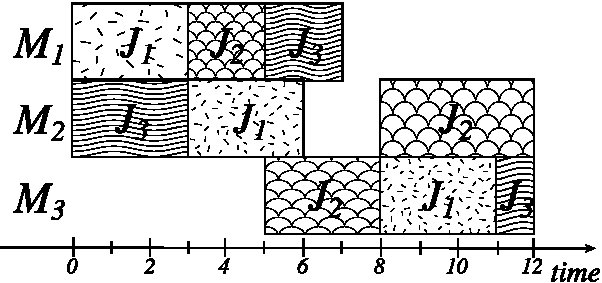
\includegraphics[width=0.8\linewidth]{images/gantt-charrt.pdf}\\
    Figure 1.1: Gantt-Chart of a solution for a 3x3 problem in table 1.1, reproduced from \cite{YamadaNakanoJSSP}
\end{center}

\subsection{JSSP as a disjunctive graph} \label{JSSP as a disjunctive graph}

JSSP can be represented by a disjunctive graph \cite{YamadaNakanoJSSP, BLAZEWICZ2000317} $G = ( O, A \cup E )$, where $O$ denotes a set of vertices corresponding to different operations $O_{ij}$ together with \textit{source} node and \textit{sink} node representing start and end of the schedule, respectively. The source node can be interpreted as a dummy operation preceding all other operations, and the sink node as a dummy operation succeeding all other operations. Both dummy operations have a processing time equal to zero. Nodes $O$ are weighted by the processing time of their corresponding operation. $A$ is a set of conjunctive arcs representing precedence constraints between operations, and between the jobs and dummy operations. $E = \bigcup_{k} E_k$ is a set of disjunctive edges, where $E_k$ is a clique connecting operations that require the same machine $M_k$ for their execution.
\begin{center}
    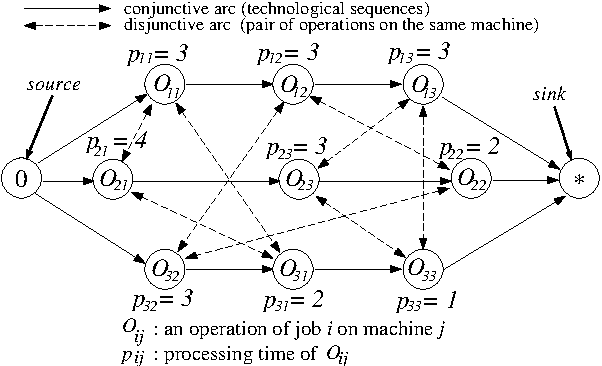
\includegraphics[width=0.75\linewidth]{images/jssp_disjunctive_graph.pdf}\\
    Figure 1.2: Disjunctive graph representation of 3x3 instance in table 1.1, retrieved from \cite{YamadaNakanoJSSP}
\end{center}

Finding a solution to the job-shop scheduling problem can be viewed as defining the ordering between operations requiring the same machine. In the disjunctive graph, this is done by turning all disjunctive edges into conjunctive arcs \cite{YamadaNakanoJSSP, BLAZEWICZ2000317} in such a way that the resulting graph is a direct acyclic graph (DAG) \cite{doi:10.1287/opre.17.6.941}. The makespan $C_\text{max}$ is then given by the longest weighted path from source to sink.

\subsection{JSSP as a heterogenous graph} \label{JSSP as a heterogenous graph}

In \cite{10226873}, authors represent JSSP as a heterogenous graph $H = (O, M, E)$, where $O$ is a set of operation nodes, $M$ is a set of machines nodes, and $E$ is a set of edges.
\par
Features of operation nodes include the status of the operation, the processing time, the remaining time of the operation, and the number of remaining operations in the current job. Features of machine nodes include the status of the corresponding machine and the remaining time of the operation being processed.
\par
Each edge can be either operation-to-operation ($O-O$) edge, machine-to-machine ($M-M$) edge, or operation-to-machine ($O-M$) edge. $O-O$ edges fully connect all operations in the same job, and all machines are fully connected via $M-M$ edges. $O-M$ edge connects operations with machines on which they can be processed.

\section{Flexible Job-shop Scheduling Problem}

FJSP is an extended version of JSSP with the only difference being that each operation $O_{ij} \in \mathcal{O}$ can be processed on any machine $M_k$ from the given subset of machines $\mathcal{M}_{ij} \subseteq \mathcal{M}$ with processing time $p_{ijk}$ \cite{9826438}. Solving FJSP then consists of selecting the appropriate machine for each operation (machine selection) and determining its start time (operation sequencing) \cite{https://doi.org/10.1049/iet-cim.2018.0009}. 

\subsection{FJSP as a disjunctive graph}

Similarly, as in \ref{JSSP as a disjunctive graph}, the disjunctive graph representation for the FJSP can be written as $G = (O, A, E)$ \cite{Brandimarte_1993, 9826438, LEI2022117796}, where $O$ is a set of nodes representing operations and two dummy operations representing start and end, $A$ is a set of conjunctive arcs representing precedence constraints between operations, and $E = \bigcup_{k} E_k$ is a set of disjunctive edges. The only difference with respect to JSSP is that each operation can be part of multiple cliques. An example of disjunctive graph representation for FJSP is shown in Figure 1.3.
\begin{center}
    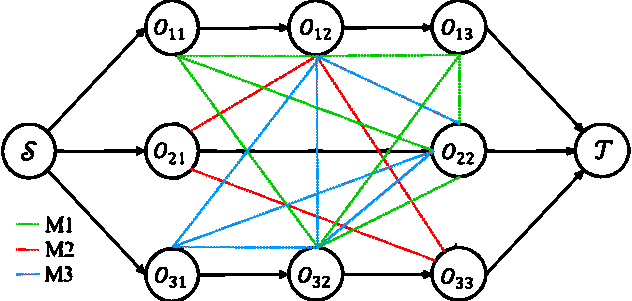
\includegraphics[width=0.75\linewidth]{images/fjsp_disjunctive_graph.pdf}\\
    Figure 1.3: Disjunctive graph representation of FJSP, reproduced from \cite{LEI2022117796}
\end{center}

\subsection{FJSP as a heterogenous graph}

In \cite{9826438}, authors represent FJSP as a heterogenous graph defined as $H = (O, M, A, \Sigma)$. Set of operation nodes $O$ and set of conjunctive arcs $A$ is the same as in the disjunctive graph. A set of machine nodes $M$ is added representing machines, and a set of disjunctive edges $E$ is replaced by a set of $O-M$ edges $\Sigma$ connecting operation nodes and machine nodes. An example of a heterogeneous graph for FJSP is shown in Figure 1.4 \cite{9826438}.
\begin{center}
    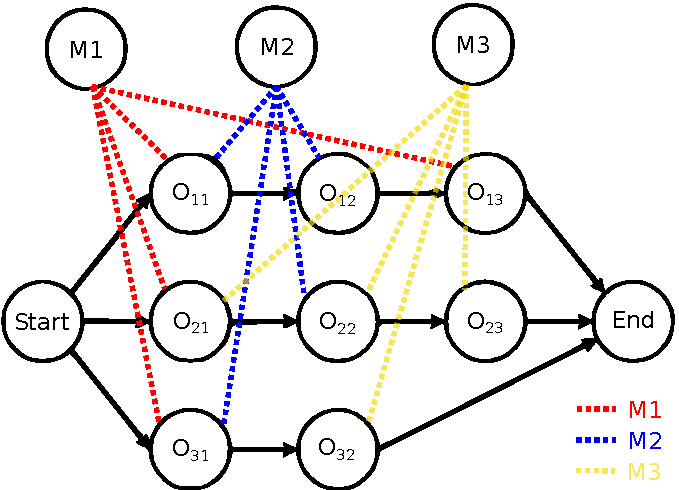
\includegraphics[width=0.75\linewidth]{images/fjsp_heterogenous_graph.pdf}\\
    Figure 1.4: Heterogeneous graph of FJSP, reproduced from \cite{LEI2022117796}
\end{center}

\section{Dynamic job-shop scheduling problem}

Dynamic job-shop scheduling problem (DJSP) is a dynamic version of JSSP where $n$ jobs are known at the beginning of the schedule, i.e., the start time of the first operation is $S_{ij} \geq 0$, and $n'$ jobs arrive after the start of the schedule, i.e., the corresponding start time is $S_{ij} \geq t_a$, where $t_a > 0$ is time of arrival \cite{KUNDAKCI201631, Haupt_1989a}.

\section{Priority Dispatching Rules}
Priority dispatching rules (PDRs) are a greedy heuristic method for solving JSSP in $\left|\mathcal{O}\right|$ steps \cite{zhang2020learning}. Each step identifies a set of eligible operations by selecting unscheduled operations whose precedent operation has already been scheduled. Then, for each eligible operation, PDR computes a priority index and selects the one with the highest priority to be dispatched \cite{zhang2020learning}. The start time must also be determined for the selected operation, but it is sensible to start it as soon as possible \cite{discovering_dispatching_rules}. In FJSP, PDR also selects the machine by computing the priority index for each eligible machine after selecting an operation.
\par
Traditional PDRs compute the priority index based on the set of features for each operation \cite{Haupt_1989a}. In the literature, many PDRs have been studied over time \cite{7232991, discovering_dispatching_rules, doi:10.1080/00207543.2011.611539, Haupt_1989a}. In this thesis, only a few of them will be mentioned, notably \cite{Haupt_1989a, 10226873}:
\begin{itemize}
    \item \textit{First in first out} (FIFO) - select earliest available operation 
    \item \textit{Most operation remaining} (MOR) - select operation of a job with most remaining operations
    \item \textit{Shortest process-time} (SPT) - select operation with shortest processing time $p_{ij}$
    \item \textit{Most work remaining} (MWKR) - select operation of a job with the largest sum of processing times $p_{ij}$ of remaining operations
\end{itemize}
As mentioned in \ref{JSSP as a disjunctive graph}, solving job scheduling can be viewed as turning each disjunctive edge into the conjunctive arc. Decisions made by PDRs can then be viewed as actions changing the disjunctive graph. This process can then be formulated as a Markov Decision Process (MDP) \cite{zhang2020learning, jssp_rl_env}, allowing PDRs to be learned automatically via (deep) reinforcement learning techniques.

\subsection{MDP for JSSP}

MDP is a stochastic decision-making process defined as a tuple $(\mathcal{S}, \mathcal{A}, \mathcal{R}, \mathcal{P}, \gamma)$, where $\mathcal{S}$ is a finite set of possible states, $\mathcal{A}$ is the set of possible actions, $\mathcal{R}$ is the reward function,  $\mathcal{P}$ is the transition probability, and $\gamma$ is the discount factor \cite{10226873, jssp_rl_env}. 
\par
\textit{State} $S_t \in \mathcal{S}$ at timestep $t$ is a graph, either a disjunctive graph presented in \ref{JSSP as a disjunctive graph} \cite{zhang2020learning} or heterogeneous graph in \ref{JSSP as a heterogenous graph} \cite{10226873}. For the disjunctive graph, the initial state is the JSSP representation described in \ref{JSSP as a disjunctive graph}, and the final state is the disjunctive graph with all disjunctive edges $E$ turned into conjunctive arcs $A$ \cite{zhang2020learning}. For a heterogeneous graph, partial schedule $S_{ij}(t)$ is maintained, where $S_{ij}(t)$ is real dispatch time $S_{ij}$ if operation $O_{ij}$ has been already dispatched \cite{9826438}. Otherwise, $S_{ij}(t)$ is a recursive estimate calculated by precedence constraints.
\par
\textit{Action} $a_t \in \mathcal{A}$ is an eligible operation at time step $t$. Since there is at most one eligible operation from each job, action space is $\left|\mathcal{J}\right|$ \cite{zhang2020learning}.
\par
A state transition from state $S_t$ to $S_{t+1}$ after executing $a_t$ in the disjunctive graph is done by updating the direction of the corresponding disjunctive edge \cite{zhang2020learning}. Schedule $S_{ij}(t)$ and node features are updated in a heterogeneous graph. An example of a transition in the disjunctive graph is shown in Figure 1.5 below \cite{zhang2020learning}.

\textit{Reward} for each action is the difference between the makespan $C_\text{max}(s_t)$ at timestep $t$ and $C_\text{max}(s_{t+1})$ at timestep $t+1$. Summing over all rewards given $\gamma = 1$ gives us \textit{cumulative reward} $C_\text{max}(s_0) - C_\text{max}(s_{\left|\mathcal{O}\right|})$, where $C_\text{max}(s_{\left|\mathcal{O}\right|})$ corresponds to the makespan of final schedule. Since the $C_\text{max}(s_0)$ is a constant specific to the problem instance, maximizing cumulative reward minimizes final schedule makespan $C_\text{max}$ \cite{zhang2020learning, 10226873, 9826438}. 

\subsection{MDP for FJSP}
Since solving FJSP consists of selecting both the eligible operation and choosing a compatible machine, the difference w.r.t. JSSP is that the action $a_t \in \mathcal{A}$ is a $O-M$ tuple (operation-machine) representing the choice of the operation to be dispatched, and the machine on which the operation will be processed \cite{9826438, LEI2022117796}. \\
Also, in the heterogeneous graph in the case of FJSP, when operation $O_{ij}$ is dispatched, only an $O-M$ edge corresponding to $O-M$ action tuple is kept, and other $O-M$ edges containing dispatched operation are removed.  

\chapter{Graph neural networks and deep reinforcement learning}
\label{chap:math}

Deep learning and neural networks have achieved unprecedented success since their introduction and currently are state-of-the-art in numerous fields, such as object detection \cite{DBLP:journals/corr/RedmonDGF15, 10.1109/IVS.2019.8813777, 8627998}, machine translation \cite{DBLP:journals/corr/LuongPM15, 8003957, DBLP:journals/corr/abs-2002-07526}, and many others \cite{DONG2021100379, 10.1145/3505243, PICCIALLI2021111}. Many deep learning techniques involve learning from Euclidian data (e.g., images, text, and videos). At the same time, there is an increasing number of fields where data is represented as graphs. For example, the interaction of users on social media \cite{10.1145/3308558.3313488}, atoms and their bonds in protein molecules \cite{strokach2020fast}, and traffic forecasting \cite{JIANG2022117921}. Learning from graph data has created significant challenges. Graphs can be irregular, with varying numbers of nodes, and each node can have a different number of neighbors. As a result, some important operations (e.g., convolution) can not be applied the same way as in the case of images. With growing interest in deep learning from graph data, new methods motivated by Convolutional Neural Networks and Recurrent Neural networks have been developed. For example, an image can be thought of as a graph, where each node is a pixel, and edges connect nodes partaking in convolution, as illustrated in Figure 2.1 below \cite{9046288}.\\
\begin{center}
    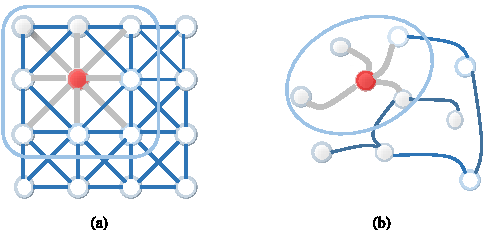
\includegraphics[width=0.6\linewidth]{images/image_vs_graph.pdf}\\
    Figure 2.1: 2-D Convolution versus graph convolution \cite{9046288}
\end{center}
\newpage
Similarly, for text processing and RNNs, text can be thought of as a graph, where each node is a word in a sentence, and every two consecutive words are connected via an oriented arc, as illustrated in Figure 2.2 below \cite{sanchez-lengeling2021a}.
\begin{center}
    
\includegraphics[width=0.7\linewidth]{images/graph_are_all_around_us.pdf}\\
    Figure 2.2: Text as a graph, reproduced from \cite{sanchez-lengeling2021a}
\end{center}

\section{Graph Neural Networks}

In the simplest case, when data is represented as a non-oriented graph $G = (O, E)$, each node $o \in O$ has a set of features $\vec{x}_o$. For example, the processing time of each operation node in the JSSP disjunctive graph. 
\par
The Graph Neural Network (GNN) takes this graph as an input and processes its features in two phases. The first phase, called \textit{message passing phase} \cite{pmlr-v70-gilmer17a}, runs for $K$ steps and uses a message function $M_{(k)}$ and a node update function $U_{(k)}$. In each step $k$, for each node $o$, a message $\vec{m}_o^{(k + 1)}$ is calculated, and the embedding of the node $\vec{h}_o^{(k)}$ is updated according to \cite{pmlr-v70-gilmer17a}
\begin{equation}\label{equation:2.1}
	\vec{m}_o^{(k + 1)} = \sum_{w \in \mathcal{N}(o)} M_{(k)} \left(\vec{h}_o^{(k)}, \vec{h}_w^{(k)}, \vec{y}_{ow} \right) \hspace{2em} \forall o \in O \, ,
\end{equation}
\begin{equation}\label{equation:2.2}
	\vec{h}_o^{(k+1)} = U_{(k)} \left(\vec{h}_o^{(k)}, \vec{m}_o^{(k+1)}\right) \hspace{2em }\forall o \in O \, , 
\end{equation}
where $\mathcal{N}(o)$ in the sum defines the neighbourhood of the node $o$ in graph $G$. The initial embedding of the node is $\vec{h}_o^{(0)} = \vec{x}_o$. Each step is often called a \textit{layer} of GNN.
\par
In the \textit{readout phase}, a readout function $R$ computes a feature vector $\vec{z}_o$ from obtained node embeddings \cite{pmlr-v70-gilmer17a}
\begin{equation}\label{equation:2.3}
	\vec{z}_o = R\left(\vec{h}_o^{(K)}\right) \hspace{2em} \forall o \in O \, .
\end{equation}
Message function $M_{(k)}$, node update function $U_{(k)}$, and readout function $R$ can all be parametrized differentiable functions. Each layer can have different parameters for these functions.
\par
Different forms of equations \ref{equation:2.1}, \ref{equation:2.2}, and \ref{equation:2.3} lead to different types of GNNs performing different tasks, for example, Graph Convolutional Neural Networks, Graph Recurrent Neural Networks, and Graph Attention Networks \cite{sanchez-lengeling2021a, 10.1145/3495161, DBLP:journals/corr/abs-1810-00826}. This thesis will focus primarily on relevant GNN architectures used in available job scheduling models described in the next chapter, specifically Graph Isomorphism Network and Graph Attention Network.

\subsection{Graph Isomorphism Network} \label{graph Isomorphism network}
Graph Isomorphism Network (GIN) is a GNN variant achieving maximum discriminative power \cite{DBLP:journals/corr/abs-1810-00826}, i.e., it has as large discriminative power as the Weisfeiler-Leman graph isomorphism test for the existence of an isomorphism between two graphs $G$ and $H$ \cite{leman1968reduction}. Given non-oriented graph $G = (O, E)$, in the message passing phase, the update function $U_{(k)}$ is represented by a multi-layer perceptron $\text{MLP}^{(k)}$ and \ref{equation:2.2} has the following form \cite{DBLP:journals/corr/abs-1810-00826}
\begin{equation} \label{equation:2.4}
	\vec{h}_o^{(k+1)} = \text{MLP}^{(k)} \left ( \left ( 1 + \epsilon^{(k)} \right ) \vec{h}_o^{(k)} + \sum_{w\in \mathcal{N}(o)} \vec{h}_w^{(k)} \right ) \, ,
\end{equation}
where $\epsilon^{(k)}$ can be learned or a fixed scalar \cite{DBLP:journals/corr/abs-1810-00826}. In the readout phase, the readout function $R$ depends on the model's given task, e.g., node classification, link prediction, and graph classification \cite{DBLP:journals/corr/abs-1810-00826}. Readout functions will be specified for each model separately in the next chapter.
\par
A straightforward strategy to extend GIN to directed graphs $G = (O, A)$ is to define the neighborhood of node $o \in O$ as $\mathcal{N}(o) = \{ w | \ (w, o) \in A\}$, i.e., all incoming neighbors of $o$ \cite{zhang2020learning}.\\
\\
For GIN on heterogeneous graphs, the equation \ref{equation:2.4} is applied separately for each type of neighbor node and then combined \cite{10226873, pytorch_hetero_conv}. Let $a$ denote a type of node $o$, $b$ denote a type of node $w$, and $r$ be an edge type connecting nodes of types $a$ and $b$. Then, let neighborhood $\mathcal{N}_{r}(o)$ be a set of nodes $b$ connected to $o$ by an edge of type $r$. Then, for each edge type $r$, updated embedding $\vec{h}_{o, r}^{(k+1)}$ of node $o$ is calculated by equation \ref{equation:2.4} separately (with separate multi-layer perceptrons) as follows \cite{pytorch_hetero_conv}
\begin{equation} \label{equation:2.5}
	\vec{h}_{o, r}^{(k+1)} = \text{MLP}^{(k)}_{r} \left ( \left ( 1 + \epsilon_{r}^{(k)} \right ) \vec{h}_{o}^{(k)} + \sum_{w\in \mathcal{N}_{r}(o)} h_{w}^{(k)} \right ) \, ,
\end{equation}
where $\text{MLP}^{(t)}_{r}$ is a multilayer perceptron for edge type $r$ \cite{pytorch_hetero_conv}. New embeddings for the node for each edge type $\vec{h}_{o, r}^{(k+1)}$ are then combined via some aggregation function \cite{pytorch_hetero_conv}, for example, a sum.

\subsection{Graph Attention Network}
Graph Attention Network (GAT) is a graph neural network architecture leveraging an attention mechanism \cite{veličković2018graph}. In each step (layer) $k$, nodes assign different importance weights to different nodes in their neighborhood by attending over their features. In job scheduling, higher importance weights may be assigned to operations expected to start sooner \cite{9826438}.
\par
In the first step, \textit{attention coefficients} $e_{ij}$ are computed as follows \cite{9826438, veličković2018graph}
\begin{equation} \label{equation:2.6}
	e_{ow} = a\left ( \boldsymbol{W} \vec{h}_o^{(k)}, \boldsymbol{W} \vec{h}_w^{(k)}  \right ) \, ,
\end{equation}  
where $a$ is a shared attention mechanism, and $\boldsymbol{W}$ is a shared learnable linear transformation. Attention mechanism $a$ is usually a single-layer feedforward neural network parametrized by a learnable vector $\vec{b}$ with LeakyReLU activation \cite{9826438, veličković2018graph, DBLP:journals/corr/abs-2105-14491}
\begin{equation} \label{equation:2.7}
	e_{ow} = \text{LeakyReLU}\left ( \vec{b} \cdot \left [ \boldsymbol{W}\vec{h}_o^{(k)} || \boldsymbol{W}\vec{h}_w^{(k)} \right ] \right ) \, ,
\end{equation}
where $\bullet||\bullet$ represents concatenation.
\par
Then, the attention coefficients are normalized using the Softmax function only across the neighborhood and the node itself \cite{9826438, veličković2018graph}
\begin{equation}
	\alpha_{ow} = \frac{\exp(e_{ow})}{\sum_{q \in \mathcal{N}(o)} \exp(e_{oq})} \hspace{2em} \forall w \in \mathcal{N}(o) \cup {o} \, .
\end{equation}
As the last step, GAT computes a new node embedding as follows \cite{9826438, veličković2018graph}
\begin{equation} \label{equation:2.9}
	\vec{h}_o^{(k+1)} = \sigma \left ( \sum_{w \in \mathcal{N}(o) \cup {o}} \alpha_{ow} \boldsymbol{W} \vec{h}_w^{(k)} \right ) \, ,
\end{equation}
where $\sigma$ is an activation function. 
\par
It is also possible to use \textit{multi-head attention} to stabilize the learning process. Multiple independent attention mechanisms execute the transformation in equation \ref{equation:2.9}, and their results are aggregated by concatenation or averaging \cite{veličković2018graph}. This process is illustrated in Figure 3.1 below \cite{veličković2018graph}.
\begin{center}
    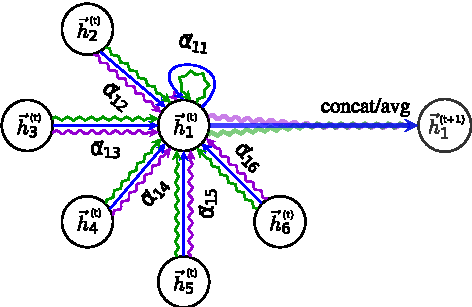
\includegraphics[width=0.5\linewidth]{images/graph_attention_network_pdfa.pdf}\\
	Figure 3.1: Illustration of multi-head attention with three heads. Different arrow colors denote independent attention mechanisms. Reproduced from \cite{veličković2018graph}
\end{center}
\par
One straightforward strategy to extend GAT on heterogeneous graphs is constructing separate learnable linear transformation $\boldsymbol{W}_{b_i}$ for each node type $b_i$ in equations \ref{equation:2.6}, \ref{equation:2.7}, \ref{equation:2.9}, projecting each node type to a shared latent space with the same dimension.

\section{Deep reinforcement learning}

Given MDP tuple $(\mathcal{S}, \mathcal{A}, \mathcal{R}, \mathcal{P}, \gamma)$ as described in \ref{MDP for JSSP}, at each time step $t$, the agent receives a state $s_t \in \mathcal{S}$, selects an action $a_t \in \mathcal{A}$ following a policy $\pi(a_t|s_t)$, receives a reward $r_t$ and a new state $s_{t+1}$ according to the probability distribution $\mathcal{P}(s_{t+1} | s_t, a_t)$, and the cycle repeats \cite{DBLP:journals/corr/Li17b}. A sequence of states, actions, and rewards is called a trajectory. The discounted cumulative reward of the trajectory with length $T$ starting at time $t$ is the sum $G_t = \sum_{k=0}^T \gamma^k r_{t+k}$. The probability of the trajectory is $P_t = \Pi_{k=0}^T \mathcal{P}(s_{t+k+1} | s_{t+k}, a_{t+k})$. The goal of an agent is to maximize the expected discounted cumulative reward $\mathbb{E}[G_t]$ over all possible trajectories \cite{DBLP:journals/corr/Li17b}. Long term value of a state $s$ defined as $v(s) = \mathbb{E}\left [ G_t | s_t = s \right ]$ is the expected cumulative reward from the state $s$ following policy $\pi$. An optimal state value $v_*(s) = \max_\pi v_\pi(s)$ is the maximum achievable value for the state $s$. For the optimal state value, the Bellman equation holds \cite{DBLP:journals/corr/Li17b}
\begin{equation}
	v_*(s) = \max_a \sum_{s'} \mathcal{P} (s' | s,a)\left [ \mathcal{R}(s, a) + \gamma v_*(s') \right ] \, .
\end{equation}
The action-value function $q_\pi(s,a) = \mathbb{E} \left [ G_t | s_t=s, a_t=a\right ]$ is the expected cumulative reward after taking an action $a$ in state $s$ following policy $\pi$. The optimal action-value function $q_* (s,a) = \max_\pi q_\pi(s, a)$ is the maximum state-action value possible for given state $s$ and action $a$. Policy maximizing $q_\pi(s,a)$ and $v_\pi(s)$ is called optimal policy and is denoted as $\pi_*$ \cite{DBLP:journals/corr/Li17b}.
\par
Traditional algorithms for finding optimal policies include value iteration \cite{barto1989learning}, policy iteration \cite{Howard1960DynamicPA}, temporal difference learning \cite{tesauro1995temporal}, Q-learning \cite{watkins1992q}, and SARSA \cite{sarsa}.
\par
Deep reinforcement learning (DRL) methods use deep neural networks to approximate reinforcement learning components, such as value function $\hat{v}(s)$, action-value function $\hat{q}(s, a)$, policy $\pi(a|s)$, and also possibly state transition function and reward function  \cite{DBLP:journals/corr/Li17b}. 

\subsection{Policy optimization} \label{policy_optimization}

The policy $\pi_\theta$ can be improved by performing gradient ascent w.r.t. some loss function $L(\theta)$ \cite{openai_policy_optimization}
\begin{equation}
	\theta_{k+1} = \theta_k + \alpha \nabla_\theta L(\theta)|_{\theta_k} \,
\end{equation}
where $\alpha$ is called a learning rate, and $\nabla_\theta L(\theta)$ is called the \textbf{policy gradient}. 
\par
The goal of an agent following parameterized policy $\pi_\theta$ is to maximize expected return $\mathbb{E} \left [ G_t \right ]$. Plugging in $L(\theta) = \mathbb{E} \left [ G_t \right ]$ yields \cite{openai_policy_optimization,DBLP:journals/corr/SchulmanWDRK17}
\begin{equation} \label{equation:2.12}
	\nabla_\theta L(\theta) = \mathbb{E} \left [ \sum_i \nabla_\theta \log \pi_\theta(a_i|s_i) G_t \right ] \, ,
\end{equation}
where expectation averages over a finite batch of trajectories. The cumulative reward function $G_t$ is often replaced by the advantage function $A_t$, which describes how better the action is w.r.t. other actions of the current policy, i.e., $A_t(s_t,a_t) = q_\pi(s_t, a_t) - v_\pi(s_t)$ \cite{openai_policy_optimization}. Gradient \ref{equation:2.12} is obtained from the loss function \cite{DBLP:journals/corr/SchulmanWDRK17}
\begin{equation}
	L(\theta) = \mathbb{E} \left [ \sum_i \log \theta(a_i|s_i) A_t \right ] \, .
\end{equation}
Authors of \textbf{Proximal Policy Optimization} (PPO) algorithm \cite{DBLP:journals/corr/SchulmanWDRK17} propose the following loss function
\begin{equation}
	L(\theta) = \mathbb{E}_t \left [ \min \left( r_t(\theta) \hat{A_t} , \text{clip}(r_t(\theta), 1-\epsilon, 1+\epsilon) \hat{A_t} \right) \right ] \,
\end{equation}
where $r_t(\theta) = \frac{\pi_\theta(a_t|s_t)}{\pi_{\theta_\text{old}}(a_t|s_t)}$ is the probability ratio with $r(\theta_\text{old}) = 1$, and $\epsilon$ is a hyperparameter, which authors set to $\epsilon = 0.2$ \cite{DBLP:journals/corr/SchulmanWDRK17}. $\hat{A_t}$ is an advantage estimate \cite{DBLP:journals/corr/SchulmanWDRK17}
\begin{equation}
	\hat{A_t} = \delta_t + (\gamma \lambda) \delta_{t+1} + \cdots + (\gamma\lambda)^{T - t + 1} \delta_{T - 1} \, ,
\end{equation}
where $\delta_t = r_t + \gamma v(s_{t+1}) - v(s_t)$, $\lambda$ is a hyperparameter, and $t \in \left [ 0, T \right ]$.
\par
The full PPO algorithm is shown below \cite{DBLP:journals/corr/SchulmanWDRK17}. In each iteration, $N$ actors collect $T$ timesteps of data. Then, the surrogate loss of these $NT$ timesteps of data is calculated and parameters $\theta$ are optimized.

\begin{algorithm}[H]
	\caption{PPO, Actor-Critic Style}\label{algorithm:ppo}
	\begin{algorithmic}[1]
	\renewcommand{\algorithmicrequire}{\hspace*{\algorithmicindent}  \textbf{Input:}}
	\renewcommand{\algorithmicensure}{\hspace*{\algorithmicindent}  \textbf{Output:}}
	\Require Environment
	\Ensure Trained policy 
	\State $\pi_{\theta_\text{old}} \gets$ initialize random policy
	\For{iteration$=1,2,...$ }
		\For{actors$=1,2,...,N$}
			\State Run Policy $\pi_{\theta_\text{old}}$ in environment for $T$ timesteps
			\State Compute advantage estimates $\hat{A_1}$, ..., $\hat{A_T}$
		\EndFor
		\State Optimize $L$ wrt $\theta$, with $K$ epochs and minibatch size $M \leq NT$
		\State $\theta_{\text{old}} \gets \theta$
	\EndFor
	\State return $\pi_{\theta_\text{old}}$
\end{algorithmic}
\end{algorithm}

\subsection{Deep Q-network} \label{dqn}

Deep Q-network (DQN) is an algorithm using a neural network to approximate the action-value function $\hat{q}_\theta(s, a)$ \cite{mnih2015human}. It also stores agent's experience as tuples $e_t = (s_t, a_t, r_t, s_{t+1})$ in a data set $D_t = \{e_1, ..., e_t\}$. During training, Q-learning updates are performed on samples drawn uniformly from the agent's experience $D$ to reduce correlation in the trajectories observations \cite{mnih2015human}. The Q-learning update uses the following loss function \cite{mnih2015human}
\begin{equation} \label{equation:2.16}
	L_i(\theta_i) = \mathbb{E} \left [\left ( r + \gamma \max_{a'}\hat{q}_{\theta^-_i}(s',a') -\hat{q}_{\theta_i}(s,a) \right )^2 \right ] \, ,
\end{equation}
where expectation averages over a batch of $e_t$,
$\hat{q}_{\theta_i}(s,a)$ is the Q-network at iteration $i$, and $\hat{q}_{\theta^-_i}(s,a)$ is the target network used to compute targets at iteration $i$. The target network is updated with the Q-network parameters every $C$ step and fixed between updates. The full algorithm is shown below \cite{mnih2015human}.

\begin{algorithm}[H]
	\caption{Deep Q-learning with experience replay} \label{algorithm:dqn}
	\begin{algorithmic}[1]
	\renewcommand{\algorithmicrequire}{\hspace*{\algorithmicindent}  \textbf{Input:}}
	\renewcommand{\algorithmicensure}{\hspace*{\algorithmicindent}  \textbf{Output:}}
	\Require Emulator
	\Ensure Action-value function
	\State Initialize replay memory $D$ to capacity $N$
	\State Initialize action-value function $\hat{q}_\theta$ with random weights
	\State Initialize target action-value function $\hat{q}_{\theta^-} = \hat{q}_\theta$
	\For{episode $=1,...,M$}
		\State Initialize sequence $s_1 = \{x_1\}$ and preprocessed sequence $\phi_1 = \phi(s_1)$
		\For{t $=1,...,T$}
			\State With probability $\varepsilon$ select a random action $a_t$
			\State otherwise select $a_t = \text{argmax}_a \hat{q}_\theta(\phi(s_t), a)$
			\State Execute action $a_t$ in emulator and observe reward $r_t$ and image $x_{t+1}$
			\State Set $s_{t+1} = s_t, a_t, x_{t+1}$ and preprocess $\phi_{t+1} = \phi(s_{t+1})$
			\State Store transition $(\phi_t, a_t, r_t, \phi_{t+1})$ in $D$
			\State Sample random minibatch of transitions $(\phi_j, a_j, r_j, \phi_{j+1})$ from $D$
			\State Set $ y_j = \begin{cases} r_j & \mbox{if episode ends at step } j+1 \\ r_j + \gamma \max_{a'}\hat{q}_{\theta^-}(\phi_{j+1}, a') & \mbox{otherwise} \end{cases}$
			\State Perform a gradient descent step on $(y_j - \hat{q}_\theta(\phi_j, a_j))^2$ w.r.t to $\hat{q}_\theta$
			\State Every $C$ steps reset $\hat{q}_{\theta^-} = \hat{q}_{\theta}$
		\EndFor
	\EndFor
	\State return $\hat{q}_\theta$
\end{algorithmic}
\end{algorithm}

The max operator in equation \ref{equation:2.16}, also present in standard Q-learning algorithm \cite{watkins1992q}, uses the same action-value function to select and evaluate the action, leading to overoptimistic value estimates. To counteract this, in Double Q-learning \cite{hasselt2010double}, two value functions are learned by randomly choosing which to update. During each update, one function selects a greedy action, and the other determines its value. Using this mechanism in DQN algorithm \ref{algorithm:dqn} leads to an algorithm called \textbf{Double DQN} \label{Double DQN} \cite{Hasselt_Guez_Silver_2016} (DDQN), as a reference to both Double Q-learning and DQN. DDQN replaces expression for target $y_j$ in case \textit{"otherwise"} on line 13 in algorithm \ref{algorithm:dqn} with \cite{Hasselt_Guez_Silver_2016}
\begin{equation}
	y_j = r_j + \gamma \hat{q}_{\theta^-}(\phi_{j+1}, \text{argmax}_a \hat{q}_\theta(\phi_{j+1}, a)) \, .
\end{equation}
The Q-network selects the action, and the target network estimates its value.

\chapter{Published models}

This chapter will present five publicly available job scheduling models based on deep reinforcement learning on graph neural networks. Three models are designed for JSSP, and two are for FJSP. For models designed for JSSP, our extension to DJSP is also presented. Each presented model is named after the GitHub repository in which it was found. 

\section{JSSP Models}

\subsection{L2D} \label{l2d_model}
\textbf{L2D} is a model published in \cite{zhang2020learning}, source code was obtained from \cite{github_l2d}. To represent the JSSP, it employs a modified disjunctive graph described in \ref{JSSP as a disjunctive graph}, where the authors start with the original disjunctive graph containing only conjunctive arcs, and after each dispatched operation, they add a conjunctive arc representing new precedence constraint. This process is shown in the Figure 3.1 below \cite{zhang2020learning}. This design solves the problem: replacing each disjunctive edge with a pair of opposite conjunctive arcs results in a fully oriented graph with too many conjunctive arcs to compute the GIN efficiently \cite{zhang2020learning}.
\par
To parametrize the policy $\pi_\theta(a_t|s_t)$, GIN for oriented graphs described in \ref{graph Isomorphism network} is used to obtain graph node embeddings $\vec{h}_o^{(K)}$ in the message passing phase. Initial node features were a 2-elementer vector $\vec{h}_o^{(0)} = (I(o), C_{LB}(o))$, where $I(o)$ is equal to 1 only if $o \in O$ is scheduled, otherwise 0, and $C_{LB}(o)$ is the lower bound of the estimated time of completion. 
\par
To select the action $a_t$ at $s_t$ in the readout phase, obtained graph embeddings are pooled using average pooling, i.e., $\vec{h}_G = \frac{1}{|O|} \sum_{o \in O} \vec{h}_o^{(K)}$, concatenated with the embedding of the eligible operation $o$ corresponding to the action $a_t$, and passed through a multi-layer perceptron to obtain a score for the corresponding action $scr(a_t) = \text{MLP}_{\pi_\theta}\left ( \left [h_o^{(T)} || h_G \right ] \right )$. The softmax function is then applied to obtain a distribution over available actions $P(a_t)$ from the scores \cite{zhang2020learning}. Selected action is started as soon as possible. To train the policy, authors used PPO discussed in \ref{policy_optimization}.
\begin{center}
    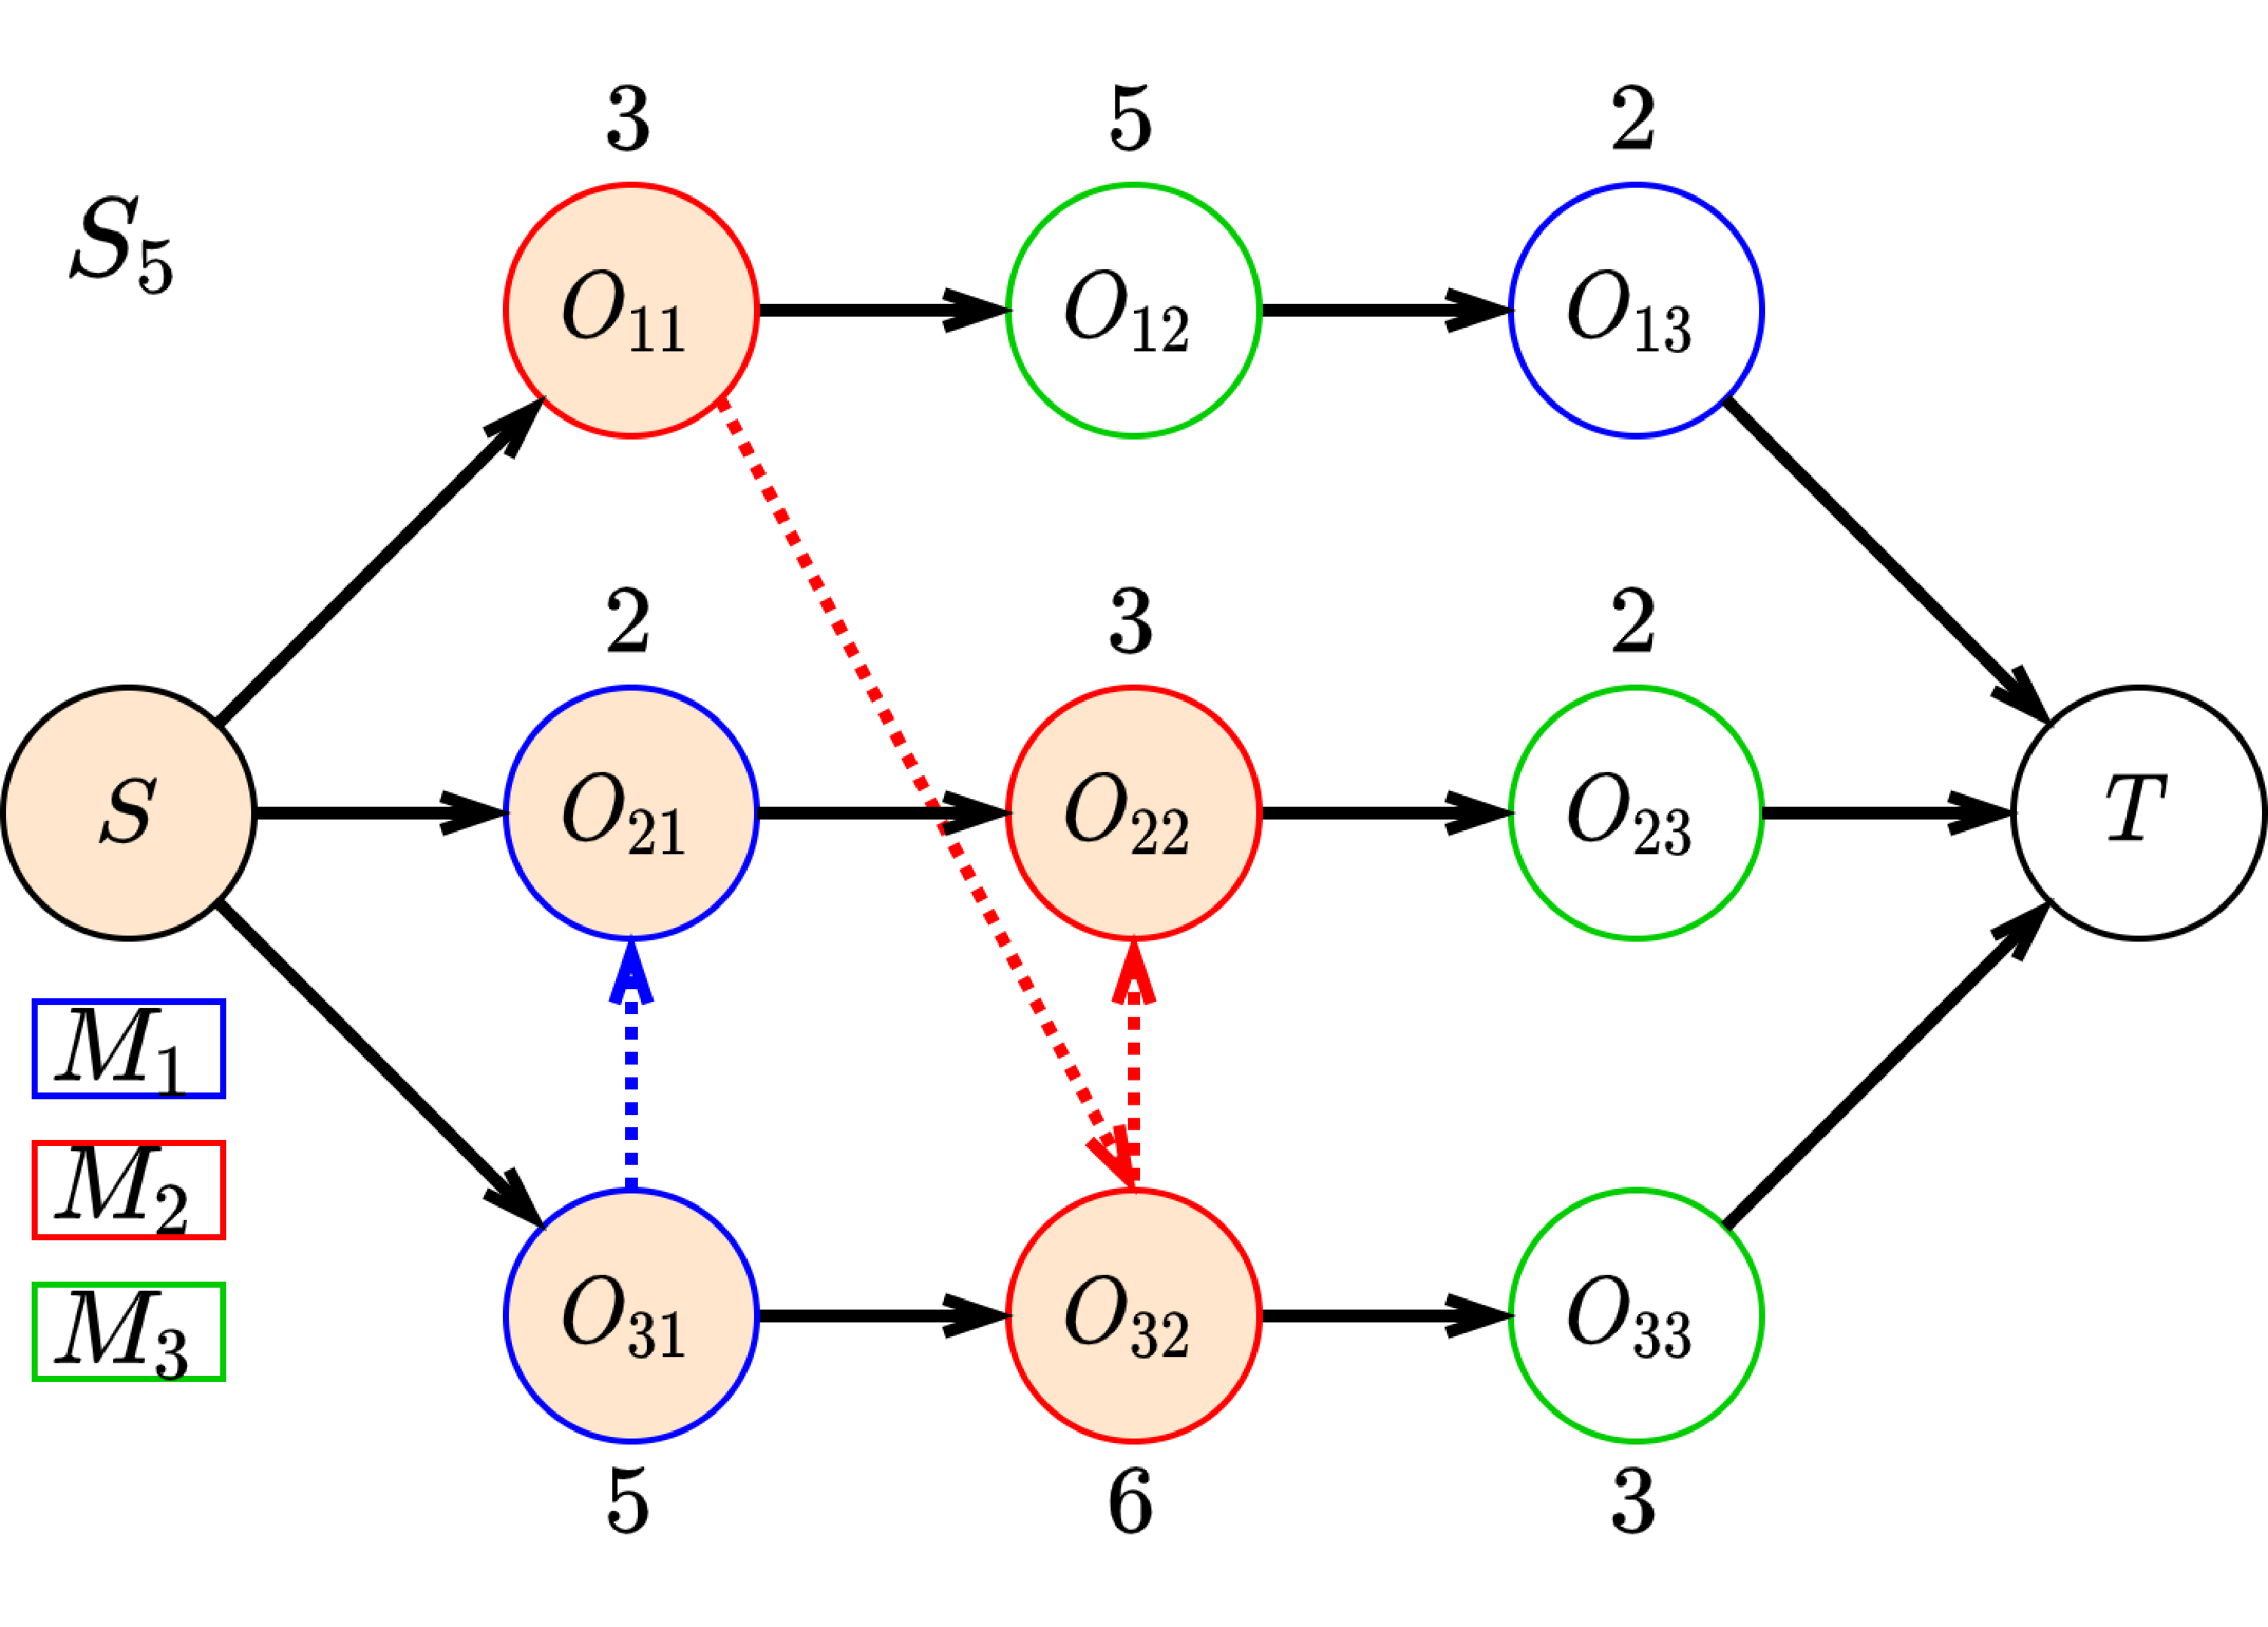
\includegraphics[width=0.75\linewidth]{images/jssp_adding_arcs.pdf}\\
    Figure 3.1: Disjunctive graph with original precedence constraints (black arrows), and three precedence constraints (red and blue arrows) between already scheduled operations (orange circles). Reproduced from \cite{zhang2020learning}.
\end{center}

\subsubsection{Dynamic L2D}

Since \textbf{L2D} is a model developed strictly for JSSP, we had to extend it to apply to DJSP. The main idea behind our algorithm is that when a new job $J_\text{new}$ arrives with the arrival time $t_a$, we want to reschedule all operations that have not started yet. To do this, we keep track of currently known jobs $J_\text{known}$, and a list of already started operations ($S_{ij} < t_a$) called \textit{plan}. When rescheduling, we first formulate the JSSP instance from known jobs and dispatch operations from the plan. By doing this, we get a partially solved JSSP with all operations with $S_{ij} \geq t_a$ removed. Then, we let \textbf{L2D} select operations to dispatch and enforce the lower bound for start time $S_{ij} \geq  t_a$. We repeat this until some termination criteria are not met; for example, no new jobs are expected. The complete algorithm written in pseudocode is shown in Algorithm \ref{algorithm:l2d}.

\begin{algorithm}
	\caption{Dynamic \textbf{L2D}} \label{algorithm:l2d}
	\begin{algorithmic}[1]
    \renewcommand{\algorithmicrequire}{\hspace*{\algorithmicindent}  \textbf{Input:}}
    \renewcommand{\algorithmicensure}{\hspace*{\algorithmicindent}  \textbf{Output:}}
    \Require Jobs known at the start $J_\text{known}$, $queue$ with arriving jobs
    \Ensure Dynamic schedule
    \State $plan \gets$ initialize empty list of actions 
    \State $instance \gets$ formulate JSSP instance from $J_\text{known}$
    \State $solution \gets$ dispatch operations in $instance$ with \textbf{L2D} 
	\While{termination criteria not met}
        \State $J_\text{new} \gets$ check if new job arrived in $queue$
        \If{$J_\text{new} = \emptyset$}
            \State \textbf{continue}
        \EndIf
		\For{operation $O_{ij}$ in $solution$}
            \If{$S_{ij} < t_a$ and $O_{ij}$ not in $plan$}
                \State add $O_{ij}$ to the $plan$
            \EndIf
		\EndFor
        \State add $J_\text{new}$ to $J_\text{known}$
        \State $instance \gets$ formulate JSSP instance from $J_\text{known}$
        \For{operation $O_{ij}$ in $plan$}
            \State dispatch $O_{ij}$ in $instance$
        \EndFor
        \State $solution \gets$ dispatch the rest of $instance$ with \textbf{L2D} and constraint $S_{ij} \geq t_a$ 
	\EndWhile
    \State return $solution$
\end{algorithmic}
\end{algorithm}

\subsection{Wheatley}

\textbf{Wheatley} is an open-source model published in \cite{wheatley}, with source code available on GitHub \cite{github_wheatley}. It is designed not only for JSSP but also for resource-constrained project scheduling problems (RCPSPs). It has been motivated by the model \textbf{L2D} and by \cite{DBLP:journals/corr/abs-2104-03760}. It has many features beyond this thesis's scope. It supports scheduling for problems with bounded but uncertain durations and offers GNN architectures beyond those described in chapter \ref{chap:math}, e.g., Principal Neighbourhood Aggregation \cite{DBLP:journals/corr/abs-2004-05718}, Directional Graph Networks \cite{DBLP:journals/corr/abs-2010-02863}, Graph convolutional networks \cite{DBLP:journals/corr/abs-2007-02133}.
\par
JSSP is represented by a disjunctive graph described in \ref{JSSP as a disjunctive graph} with \textit{"arc adding scheme"} similar to \textbf{L2D}, i.e., it starts with the graph only containing conjunctive arcs representing precedence constraints between operations in the same job. New conjunctive arcs are added during scheduling. Node features include task completion times, a boolean feature representing if the operation has already been scheduled similarly to $I(o)$ in \textbf{L2D}, one-hot encoded machine id, a boolean feature representing if the operation is selectable. The rest can be selected from the list of options, where we selected the processing time of the operation.
\par
GNN used to obtain graph node embeddings can be chosen from multiple architectures. For this thesis, we have chosen GIN described in \ref{graph Isomorphism network} so that we can compare \textbf{Wheatley} with \textbf{L2D}. For the same reason, we have chosen average pooling after extracting the embeddings.
\par
In the readout phase, \textbf{Wheatley} passes extracted graph and node embeddings through an MLP to obtain the log-odds for each eligible operation.
\par
To train the agent, \textbf{Wheatley} uses the PPO algorithm discussed in \ref{policy_optimization}.

\subsubsection*{Dynamic Wheatley} \label{dynamicwheatley}
To extend Wheatley to DJSP, we consulted Wheatley's authors in the Github issue \cite{github_wheatley_djsp}. To enforce the arrival time of the job $t_a$, we were advised to add a "virtual" operation at the start of the job with processing time $t_a$ being processed by a "virtual" machine. To avoid different jobs interfering with each other, we add one "virtual" machine per one "virtual" operation.

\subsection{IEEE-ICCE-RL-JSP} \label{model_iee_icce_rl_jsp}

\textbf{IEEE-ICCE-RL-JSP} was published in \cite{10226873}, code was obtained from Github repository \cite{github_ieee_icce_rl_jsp}. Its authors represent JSSP as a heterogeneous graph discussed in \ref{FJSP as a heterogenous graph}. In each step, this model chooses one of the traditional PDRs to determine the operation to dispatch.
\par
To parametrize the policy, the authors used GIN on heterogeneous graphs discussed in \ref{graph Isomorphism network} in the message passing phase. The features of operation nodes include the status of the operation, the processing time, the remaining time of the operation, and the number of remaining operations in the current job. The features of machine nodes include the status of the corresponding machine and the remaining time of the operation being processed \cite{10226873}.
\par
In the readout phase, obtained embeddings are pooled using sum pooling and fed into a value network based on DDQN discussed in \ref{dqn}, which outputs a score value for each PDR. The agent selects a PDR with the maximum score to determine which operation to dispatch \cite{10226873}.

\subsubsection{Dynamic IEEE-ICCE-RL-JSP}

After the inspection of the source code \cite{github_ieee_icce_rl_jsp} published in \cite{10226873}, we discovered that the authors already had prepared the functionality for setting the arrival time of the job, but it was not described in the paper itself \cite{10226873}. Therefore, we only needed to modify the source code to be able to pass job arrival times to the model. 
\par
\textbf{IEEE-ICCE-RL-JSP} takes a list of jobs and their arrival times as an input. When the model chooses which operation to dispatch, operations from jobs that have not yet arrived are not listed as eligible operations, i.e., job arrival time $t_a$ is greater than the current time.

\section{FJSP Models}

\subsection{End-to-end-DRL-for-FJSP} 

\textbf{End-to-end-DRL-for-FJSP} was published in \cite{LEI2022117796}, source code was obtained from \cite{github_end_to_end_drl_for_fjsp}. The authors represented the FJSP as a disjunctive graph discussed in \ref{FJSP as a disjunctive graph}. To reduce the computational complexity, they used the \textit{"adding arc scheme"} similar to the authors of \textbf{L2D}. This process for FJSP is shown in Figure 3.2 below.
\begin{center}
    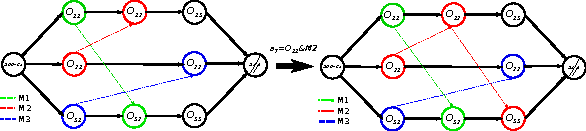
\includegraphics[width=\linewidth]{images/fjsp_adding_arcs.pdf}\\
    Figure 3.2: Action $a_7$ dispatches $O_{33}$ on $M2$ by adding a red arc corresponding to $M2$ and changing the color of $O_{33}$ to red. Reproduced from \cite{LEI2022117796}.
\end{center}
In the message passing phase, the authors use GIN, discussed in \ref{graph Isomorphism network}. Extracted operation node embeddings $\vec{h}_o^{(K)}$ are pooled using average pooling $\vec{h}_G = \frac{1}{|O|} \sum_{o \in O} \vec{h}_o^{(K)}$ as in \textbf{L2D}. The input features of each operation node are the same as in \textbf{L2D}, i.e., $\vec{h}_o^{(0)} = (I(o), C_{LB}(o))$, where $I(o)$ is equal to 1 only if $o \in O$ is scheduled, otherwise 0, and $C_{LB}(o)$ is the lower bound of the estimated time of completion.
\par
Resulting operation node embeddings do not include machine information. The authors adopt a fully connected layer to encode the state of the machine into machine embeddings $\vec{h}_m$. Those machine embeddings are then pooled to obtain a machine pooling vector $\vec{u}_m$. The input features for each machine form a vector $\vec{h}^{(0)}_k = \left ( T_k,p_{ijk}\right )$, where $T_k$ is a completion time for machine $k \in \mathcal{M}$, and $p_{ijk}$ is the processing time of operation $O_{ij}$ if its compatible with the machine $k \in \mathcal{M}$, otherwise it's an average processing time averaging over the set of compatible machines. 
\par
To select the action in the readout phase, two decoders based on multi-layer perceptrons with the same structure. Each decoder computes a probability distribution over the operation and machine space, respectively. In the first step, each decoder computes an operation score $c^o_{v}$ and machine score $c^m_{k}$ \cite{LEI2022117796}
\begin{equation}
    c^{o}_v = \text{MLP}_{\pi_{\theta}(o)} \left ( \vec{h}_v^{(K)} || \vec{h}_G || \vec{u}_m \right ) \hspace{2em} \forall v \in O \, ,
\end{equation}
\begin{equation}
    c^{m}_k = \text{MLP}_{\pi_{\theta}(m)} \left ( \vec{h}_k || \vec{h}_G || \vec{u}_m \right ) \hspace{2em} \forall k \in \mathcal{M} \, .
\end{equation}
To avoid dispatching non-eligible operations and selecting incompatible machines, their corresponding scores are set to $-\infty$. Operation scores and machine scores are then normalized by a softmax function as follows \cite{LEI2022117796}
\begin{equation}
    p_i (a_o) = \frac{e^{c^o_i}}{\sum_v e^{c^o_v}} \, ,
\end{equation}
\begin{equation}
    p_j (a_m) = \frac{e^{c^m_j}}{\sum_k e^{c^m_k}} \, ,
\end{equation}
where $p_i (a_o)$ is the probability of selecting the operation $i \in O$, and $p_j (a_m)$ is the probability of selecting the machine $j \in \mathcal{M}$.\\
\par
To train the agent, the authors propose a multi-agent version of the PPO algorithm discussed in \ref{policy_optimization}. In this case, the job operation actor makes job operation action-selection using stochastic policy $\pi_{\theta_o}(a_o|s)$, and the machine actor makes machine action-selection using a stochastic policy $\pi_{\theta_m}(a_m | s, a_o)$. A single critic network with parameters $\phi$ works as an estimator to learn the approximate state-value function $\hat{v}_\phi(s)$, which is used to calculate variance-reduced advantage function estimator $\hat{A}$. The job operation/machine actor network tries to optimize loss function $L(\theta_k)$ in Algorithm \ref{algorithm:multippo}. The critic network is updated to minimize the Mean Squared Error (MSE) objective $L_\text{MSE}(\phi)$. The complete algorithm in pseudocode is in Algorithm \ref{algorithm:multippo} \cite{LEI2022117796}. On lines 3-12, two actors collect experience until all operations are scheduled and then calculate probability ratios. On lines 13-17, aggregate job operation actor, machine actor, and critic losses are calculated. Based on the losses, updates are performed $E_s$ times on lines 18-20. This whole process is repeated $E_t$ times. The multi-PPO outputs parameters of the two trained actor networks.

\begin{algorithm}
	\caption{Multi-PPO for \textbf{End-to-end-DRL-for-FJSP}} \label{algorithm:multippo}
	\begin{algorithmic}[1]
	\renewcommand{\algorithmicrequire}{\hspace*{\algorithmicindent}  \textbf{Input:}}
	\renewcommand{\algorithmicensure}{\hspace*{\algorithmicindent}  \textbf{Output:}}
	\Require Number of training steps $E_t$, PPO update steps $E_s$, batch size $B$; training actor networks $\pi_{\theta_k} (k \in \{o,m\})$, and behavior actor networks $\pi_{\theta^\text{old}_k} (k \in \{ o,m\})$ with trainable parameters $\theta_k$ and $\theta^\text{old}_k (k \in \{ o,m \})$; critic network $\hat{v}_\phi$ with trainable parameters $\phi$; policy loss coefficient $c_p$; value functon loss coefficient $c_v$; entropy loss coefficient $c_e$; clipping parameter $\epsilon$
	\Ensure Trained parameter sets $\theta_k (k \in \{ o,m \})$ of the job/machine actor
	\State Initialize $\theta_k$ and $\phi$; $\theta_k \rightarrow \theta^\text{old}_k$ 
	\For{e $=1,...,E_t$}
		\State Sampling $B$ FJSP instances from a uniform distribution;
		\For{b $=1,...,B$}
            \For{t $=0,1,2,...$}
			\State Sample $a_{b,t}^k$ based on $\pi_{\theta_{k,\text{old}}} \left( a_{b,t}^k | s_{b,t}\right)$
			\State Observe reward $r_{b,t}$ and next state $s_{b,t+1}$;
			\State $\hat{A}_{b,t} = \sum_{t'=t}^T\gamma^{t'}r_{b,t'} - \hat{v}_\phi(s_{b,t}); \delta_{b,t}^k(\theta_k) = \frac{\pi_{\theta_k}\left(a^k_{b,t} | s_{b,t}\right)}{\pi_{\theta_{k,\text{old}}}\left(a^k_{b,t} | s_{b,t}\right)}$;
            \If{$s_{b,t}$ is terminal}
                \State break;
            \EndIf
            \EndFor
        \State $L_{CLIP}^{b,k}(\theta_k) = \mathbb{E} \left [ \min \{\delta_{b,t}^k(\theta_k)\hat{A}_{b,t}, \text{clip}\left( \delta_{b,t}^k(\theta_k), 1-\epsilon, 1+\epsilon\right) \hat{A}_{b,t} \} \right ]$
        \State $L_E^{b,k}(\theta_k) = \mathbb{E} \left [ \text{Entropy}\left(\pi_{\theta_k}\left(a_{b,t}^k | s_{b,t}\right)\right)\right ]$
        \State Aggregate job/machine actors Loss: $L(\theta_k) = c_p L_\text{CLIP}^{b,k}(\theta_k) + c_e L_e^{b,k}(\theta_k)$
        \State Aggregate critic Loss: $L_\text{MSE}(\phi)=(r_t, \hat{v}_\phi(s_t))$
		\EndFor
    \For{$PPO$ step $=1,...,E_s$}
        \State Update $\theta_k$ by a gradient method w.r.t. $L(\theta_k)$ 
        \State Update $\phi$ by a gradient method w.r.t. $L_\text{MSE}(\phi)$
    \EndFor
    \State $\theta_k^\text{old} \gets \theta_k$
	\EndFor
	\State return $\theta_k$
\end{algorithmic}
\end{algorithm}

\subsection{fjsp-drl} \label{model_fjsp_drl}

The model \textbf{fjsp-drl} was published in \cite{9826438}, and the source code was obtained from \cite{github_fjsp_drl}.
\par
The authors represented FJSP as a heterogeneous graph discussed in \ref{FJSP as a heterogenous graph}. They propose a two-stage embedding process to extract node embeddings in the message-passing phase called Heterogeneous Graph Neural Network (HGNN). In the first stage, using GIN discussed in \ref{graph Isomorphism network}, machine embeddings $\vec{\nu}_l^{(k)}$ are updated by aggregating the information from its neighborhood. Operation embeddings $\vec{\mu}_{ij}^{(k)}$ of operation $O_{ij} \in \mathcal{N}(M_l)$ are concatenated with edge embeddings $\vec{\lambda}_{ijl}^{(k)}$ of the corresponding $O-M$ edge connecting machine $M_l$ and operation $O_{ij}$ to obtain $\vec{\mu}_{ijl}^{(k)} = \left [ \vec{\mu}_{ij}^{(k)}||\vec{\lambda}_{ijl}\right ]$. Authors use two shared linear transformations $\boldsymbol{W}^M$ and $\boldsymbol{W}^O$ for machines and operations, respectively, to calculate attention coefficients $e_{ijl}$ as follows \cite{9826438}
\begin{equation}
    e_{ijl} = \text{LeakyRelu}\left (\vec{b} \cdot \left [ \boldsymbol{W}^M \vec{\nu}_l^{(k)} || \boldsymbol{W}^O \vec{\mu}_{ijl}^{(k)} \right ]\right ) \, .
\end{equation}
Attention coefficient $e_{ll}$ of the machine $M_l$ to itself is calculated as follows \cite{9826438}
\begin{equation}
    e_{ll} = \text{LeakyRelu}\left (\vec{b} \cdot \left [ \boldsymbol{W}^M \vec{\nu}_l^{(k)} || \boldsymbol{W}^M \vec{\nu}_l^{(k)} \right ]\right ) \, .
\end{equation}
Then, all attention coefficients $e_{ijl}$ and $e_{ll}$ are normalized using the Softmax function to get normalized attention coefficients $\alpha_{ijl}$ and $\alpha_{ll}$. New embeddings are then calculated as follows \cite{9826438}
\begin{equation}
    \vec{\nu}_l^{(k+1)} = \sigma \left ( \alpha_{ll} \boldsymbol{W}^M \vec{\nu}_l^{(k)} + \sum_{O_{ij} \in \mathcal{N}(M_l)} \alpha_{ijk} \boldsymbol{W}^O\vec{\mu}_{ijl}^{(k)}\right ) \hspace{2em} \forall M_l \in M
\end{equation}
\par
In the second stage, to update operation node embeddings, authors use five MLPs (denoted as $\text{MLP}_{\theta_i}$ for the i-th MLP). Individual MLPs are used to process embeddings of a preceding operation $\vec{\mu}_{i,j-1}^{(k)}$, succeeding operation $\vec{\mu}_{i,j+1}^{(k)}$, embedding of the operation itself $\vec{\mu}_{ij}^{(k)}$, and aggregated neighboring machine embedding $\nu_{ij}^{(k+1)} = \sum_{M_l\in\mathcal{N}(O_{ij})} \vec{\nu}_l^{(k+1)}$. Operation embedding update is then performed as follows \cite{9826438}
\begin{equation}
    \begin{split}
        \mu_{ij}^{(k+1)}  = \text{MLP}_{\theta_0} \Bigg( 
            &\text{ELU} \Big[ 
                \text{MLP}_{\theta_1}\left(\vec{\mu}_{i,j-1}^{(k)}\right) || 
                \text{MLP}_{\theta_2}\left(\vec{\mu}_{i,j+1}^{(k)}\right) || \\
                &\text{MLP}_{\theta_3}\left(\vec{\nu}_{ij}^{(k+1)}\right) || 
                \text{MLP}_{\theta_4}\left(\vec{\mu}_{ij}^{(k)}\right)
            \Big]    
        \Bigg) \, ,
\end{split}
\end{equation}
where ELU is the Exponential Linear Unit function with parameter $\alpha > 0$ defined as \cite{elu_activation} 
\begin{equation}
    \text{ELU}(x) = \begin{cases} x & \mbox{if } x > 0 \\ \alpha (\exp(x) - 1) & \mbox{if } x \leq 0 \end{cases} \, .
\end{equation}
\par
This two-stage embedding process can be thought of as one HGNN step (layer). After K steps, the final machine embeddings $\vec{\nu}_k^{(K)}$ and operation node embeddings $\vec{\mu}_{ij}^{(K)}$ are mean-pooled and concatenated. The final vector $\vec{h}_H$ is the embedding of the heterogeneous graph $H$ \cite{9826438}
\begin{equation}
    \vec{h}_H = 
        \left [
            \frac{1}{|O|}\sum_{O_{ij} \in O} \vec{\mu}_{ij}^{(K)} 
            \middle\| 
            \frac{1}{|M|}\sum_{M_k \in M} \vec{\nu}_k^{(K)}
        \right ] \, .
\end{equation}
In the readout phase, for each feasible action $a_t = (O_{ij}, M_l) \in A_t$ in state $s_t$ at step $t$, the corresponding operation node and machine embeddings are concatenated with heterogeneous graph embedding and fed into an MLP with parameters $\omega$ with a tanh activation to get the priority index \cite{9826438}
\begin{equation}
    P(a_t, s_t) = \text{MLP}_{\omega} \left [ \vec{\mu}_{ij}^{(K)} || \vec{\nu}_l^{(K)} || \vec{h}_H \right ] \, .
\end{equation}
The probability of selection action $a_t$ is obtained by applying softmax over all possible actions
\begin{equation}
    \pi_\omega (a_t|s_t) = \frac{\exp{P(a_t,s_t)}}{\sum_{a_t'\in A_t}\exp(P(a_t',s_t))} \hspace{2em} \forall a_t \in A_t \, . 
\end{equation}
Initial operation node features $\vec{\mu}_{ij}^{(0)}$ include \cite{9826438}
\begin{enumerate}
    \item  binary value indicating whether the operation has been scheduled
    \item number of neighboring machines $|\mathcal{O}_{ij}|$
    \item processing time $p_{ijk}$ if $O_{ij}$ is scheduled, otherwise $\overline{p}_{ij} = \frac{1}{|\mathcal{O_{ij}}|}\sum_k p_{ijk}$
    \item estimated or actual start time of $O_{ij}$ in the corresponding partial schedule $S_{ij}(t)$
    \item number of unscheduled operations in the job
    \item job completion time in the partial schedule $S(t)$
\end{enumerate}
\clearpage
Initial machine node features $\vec{\nu}_{l}^{(0)}$ include \cite{9826438}
\begin{enumerate}
    \item available time: time when machine $M_l$ will finish all its currently assigned operations
    \item number of neighboring operations $|\mathcal{N}(M_l)|$
    \item utilization: ratio of nonidle time to the to the total production time
\end{enumerate}
Initial $O-M$ arc features $\vec{\lambda}_{ijl}^{(0)}$ include only corresponding processing time $p_{ijl}$ \cite{9826438}.
\par
The authors used a modified version of the PPO discussed in section \ref{policy_optimization} to train the agent. The actor is the policy network $\pi_\omega$, and critic $v_\phi$ is the network that takes $h_H$ computed by HGNN as an input and predicts the value $v(s_t)$. The critic has the same structure as the actor but has a different number of inputs. The full algorithm is written in pseudocode in Algorithm \ref{algorithm:hgnnppo}. 

\begin{algorithm}
	\caption{HGNN Training procedure with PPO for \textbf{fjsp-drl}} \label{algorithm:hgnnppo}
	\begin{algorithmic}[1]
	\renewcommand{\algorithmicrequire}{\hspace*{\algorithmicindent}  \textbf{Input:}}
	\renewcommand{\algorithmicensure}{\hspace*{\algorithmicindent}  \textbf{Output:}}
	\Require HGNN network, policy network and critic network with trainable parameters $\theta$, $\omega$ and $\phi$
	\Ensure Trained parameters
	\State Sample a batch of $B$ FJSP instances
	\For{iter $=1,2,...,I$}
		\For{b $=1,2,...,B$}  \Comment{In parallel}
			\State Initialize $s_t$ based on instance $b$
            \While{$s_t$ is not terminal}
                \State Extract embeddings using HGNN
                \State Sample $a_t \sim \pi_\omega(\cdot | s_t)$
                \State Receive reward $r_t$ and next state $s_{t+1}$
                \State $s_t \gets s_{t+1}$
            \EndWhile
			\State Compute the generalised advantage estimates $\hat{A_t}$ for each step
        \State Compute  the PPO loss $L$, and optimize the parameters $\theta$, $\omega$, and $\phi$
        \State Update network parameters
        \State Validate the policy every 10 iterations
        \State Sample a new batch of $B$ FJSP instances every 20 iterations
		\EndFor
	\EndFor
	\State return $\theta_k$
\end{algorithmic}
\end{algorithm}

\chapwithtoc{Conclusion}

In this thesis, we explored the applications of graph neural networks and deep reinforcement learning to job-shop scheduling.\\
In \textbf{Chapter 1}, we defined the job scheduling problem, flexible job shop scheduling problem, and dynamic job shop scheduling problem. We also presented priority dispatching rules as a computationally fast and intuitive heuristic, and we discussed how reinforcement learning helps automate the process of designing priority dispatching rules.\\
In \textbf{Chapter 2}, we introduced the concept of graph neural networks and deep reinforcement learning. We presented different neural architectures and algorithms for training them.\\
In \textbf{Chapter 3}, we presented five publicly available models from GitHub, four of which have been published in the literature. We described their input features, their architecture, and their training algorithms. We also presented our extension of three of these models to dynamic job shop scheduling.\\
In \textbf{Chapter 4}, we presented the setup of our experiment, in which we tested all models on the same benchmark instances. Then, we presented the results of our experiment for different job shop scheduling variants.\\
In \textbf{Chapter 5}, we discussed our results. Our findings indicate that the feature selection for the neural network is more important than the network architecture. We also discussed which features may be important for each job shop scheduling variant.\\
In conclusion, this thesis presented an experimental overview and comparison of publicly available models for solving job shop scheduling using graph neural networks and deep reinforcement learning. It also lays the foundation for future research in this area.

\ifEN
\chapwithtoc{Bibliography}
\else
\chapwithtoc{Seznam použité literatury}
\fi

\printbibliography[heading=none]


\appendix
\chapter{Using CoolThesisSoftware}

Use this appendix to tell the readers (specifically the reviewer) how to use your software. A very reduced example follows; expand as necessary. Description of the program usage (e.g., how to process some example data) should be included as well.

To compile and run the software, you need dependencies XXX and YYY and a C compiler. On Debian-based Linux systems (such as Ubuntu), you may install these dependencies with APT:
\begin{Verbatim}
apt-get install \
  libsuperdependency-dev \
  libanotherdependency-dev \
  build-essential
\end{Verbatim}

To unpack and compile the software, proceed as follows:
\begin{Verbatim}
unzip coolsoft.zip
cd coolsoft
./configure
make
\end{Verbatim}

The program can be used as a C++ library, the simplest use is demonstrated in \cref{lst:ex}. A demonstration program that processes demonstration data is available in directory \verb|demo/|, you can run the program on a demonstration dataset as follows:
\begin{Verbatim}
cd demo/
./bin/cool_process_data data/demo1
\end{Verbatim}

After the program starts, control the data avenger with standard \verb-WSAD- controls.

\begin{listing}
\begin{lstlisting}
#include <CoolSoft.h>
#include <iostream>

int main() {
	int i;
	if(i = cool::ProcessAllData()) // returns 0 on error
		std::cout << i << std::endl;
	else
		std::cerr << "error!" << std::endl;
	return 0;
}
\end{lstlisting}
\caption{Example program.}
\label{lst:ex}
\end{listing}


% if your attachments are complicated, describe them in a separate appendix
%\include{attachments}

\openright
\end{document}
